% Created 2026-03-09 Mon 22:56
% Intended LaTeX compiler: pdflatex
\documentclass[bigger]{beamer}
\usepackage[utf8]{inputenc}
\usepackage[T1]{fontenc}
\usepackage[activate={true,nocompatibility},final,tracking=true,kerning=true,spacing=true,factor=1100,stretch=10,shrink=10]{microtype}
\usepackage[dvipsnames,svgnames]{xcolor}
\usepackage{hyperref}
\usepackage[utf8]{inputenc}
\usepackage{fixltx2e}
\usepackage{graphicx}
\usepackage{longtable}
\usepackage{float}
\usepackage{wrapfig}
\usepackage{rotating}
\usepackage[normalem]{ulem}
\usepackage{amsmath}
\usepackage{textcomp}
\usepackage{marvosym}
\usepackage{wasysym}
\usepackage{multicol}
\usepackage{amssymb}
\usepackage[colorlinks=true, linkcolor=DarkBlue, citecolor=BrickRed, urlcolor=DarkGreen]{hyperref}
\usepackage{minted}
\usepackage[style=apa,backend=bibtex]{biblatex}
\definecolor{purple_plain}{RGB}{94,129,172}
\definecolor{grey}{RGB}{51, 63, 72}
\definecolor{DodgerBlue4}{RGB}{16, 78, 139}
\definecolor{PaleGreen1}{RGB}{154, 255, 154}
\definecolor{darkskyblue}{RGB}{0, 103, 165}
\definecolor{darkgreen}{RGB}{0,128,0}
\definecolor{amaranth}{rgb}{0.9, 0.17,0.31}
\definecolor{ao-english}{rgb}{0.0,0.5, 0.0}
\usepackage{amsmath,amsfonts,amssymb,amsthm,enumerate,multirow,array,graphicx,lscape,lastpage,mathabx,csquotes}
\usetheme{Madrid}
\usepackage{fontawesome}
\hypersetup{linktoc = all, colorlinks = true, urlcolor = DodgerBlue4, citecolor = PaleGreen1, linkcolor = black}
\usefonttheme{professionalfonts}
\usepackage{tikz}
\usetikzlibrary{calc}
\usepackage{subfig}
\captionsetup[figure]{labelformat=empty}
\usecolortheme{seahorse}
\usepackage{appendixnumberbeamer}
\title[]{Customization of the CVA6 core}
\author[Hanan Quispe] % (optional)
{\textbf{Hanan Quispe}\inst{1}}
\institute[]
{\inst{1}%
Institut Polytechnique de Paris}
\titlegraphic {
\begin{tikzpicture}[overlay,remember picture]
\node[left=0.7cm] at (current page.335){
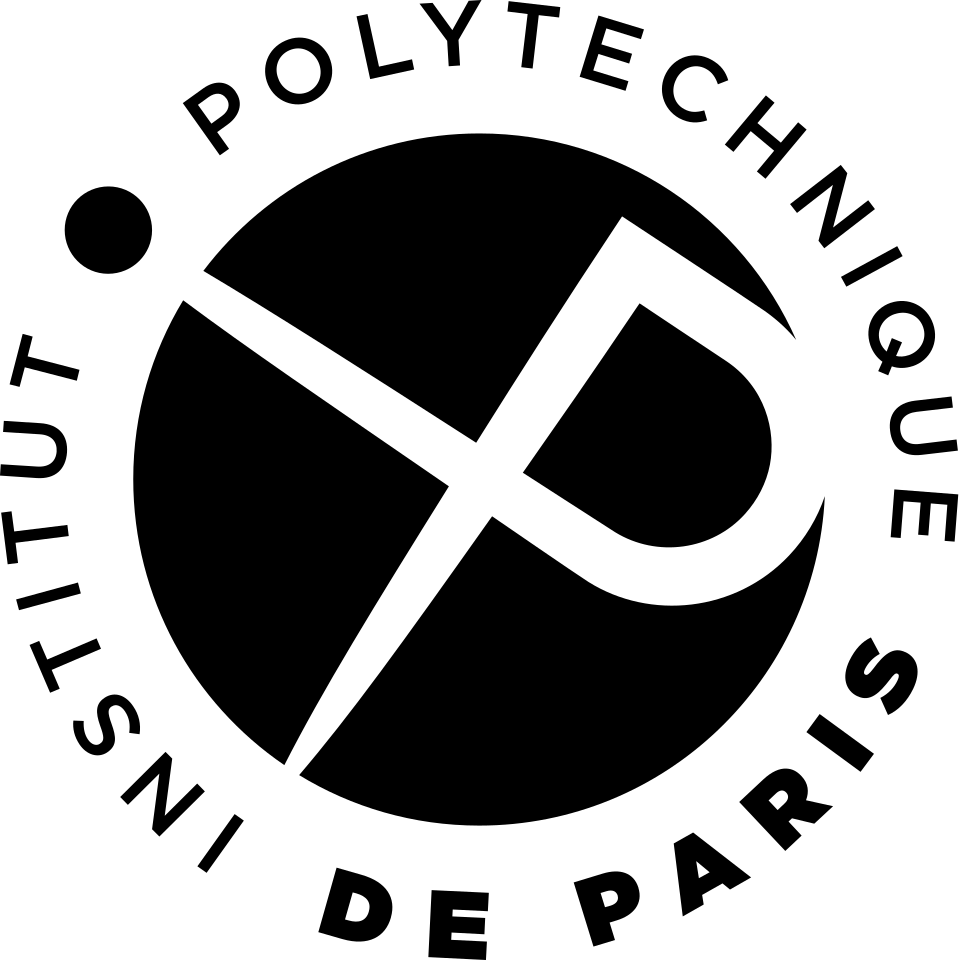
\includegraphics[width=1.8cm]{figures/logo_ip.png}};
\node[right=0.7cm] at (current page.207){

\includegraphics[width=1.5cm]{figures/logo_TSP.png}};
\end{tikzpicture}
}
\usetheme{default}
\date{March 9, 2026}
\title{Customization of the CVA6 core}
\title[PDS Research Project]{Customization of the CVA6 core}
\hypersetup{
 pdfauthor={Hanan Ronaldo Quispe Condori},
 pdftitle={Customization of the CVA6 core},
 pdfkeywords={},
 pdfsubject={},
 pdfcreator={Emacs 29.2 (Org mode 9.7.39)}, 
 pdflang={English}}
\begin{document}

\begin{frame}
    \titlepage
\end{frame}
\begin{frame}{Outline}
        \tableofcontents[hideallsubsections]
\end{frame}

\AtBeginSection[]
{
  \begin{frame}
    \frametitle{Outline}
    \tableofcontents[currentsection,hideallsubsections]
  \end{frame}
}
\section{Motivation}
\label{sec:orgcba1ffd}
\begin{frame}[label={sec:org4ec6b59}]{The CVA6 Core}
\framesubtitle{A 6-stage RISC-V Open-Source core}
\begin{columns}
\begin{column}{0.5\columnwidth}
\begin{itemize}
\item \small Industry Standard: CVA6 is a single-issue, in-order design maintained by the OpenHW Foundation (with Thales).
\item \small Versatility: Ideal for ISA extensions (Virtualization), prototyping, and integration into complex multi-core structures like OpenPiton.
\item \small Local Implementation: Internal dual-core prototype developed by the Inria Benagil team for FPGA deployment.
\end{itemize}
\end{column}
\begin{column}{0.5\columnwidth}
\begin{center}

\includegraphics[angle=0,width=4.0cm]{./figures/openhw.png}
\label{fig:openhw}
\end{center}

\begin{center}

\includegraphics[angle=0,width=5.0cm]{./figures/inria_logo.png}
\label{fig:inria}
\end{center}
\end{column}
\end{columns}
\end{frame}
\begin{frame}[label={sec:org2d2bdce}]{The CVA6 Core}
\framesubtitle{Original Single Core Version}
\begin{center}
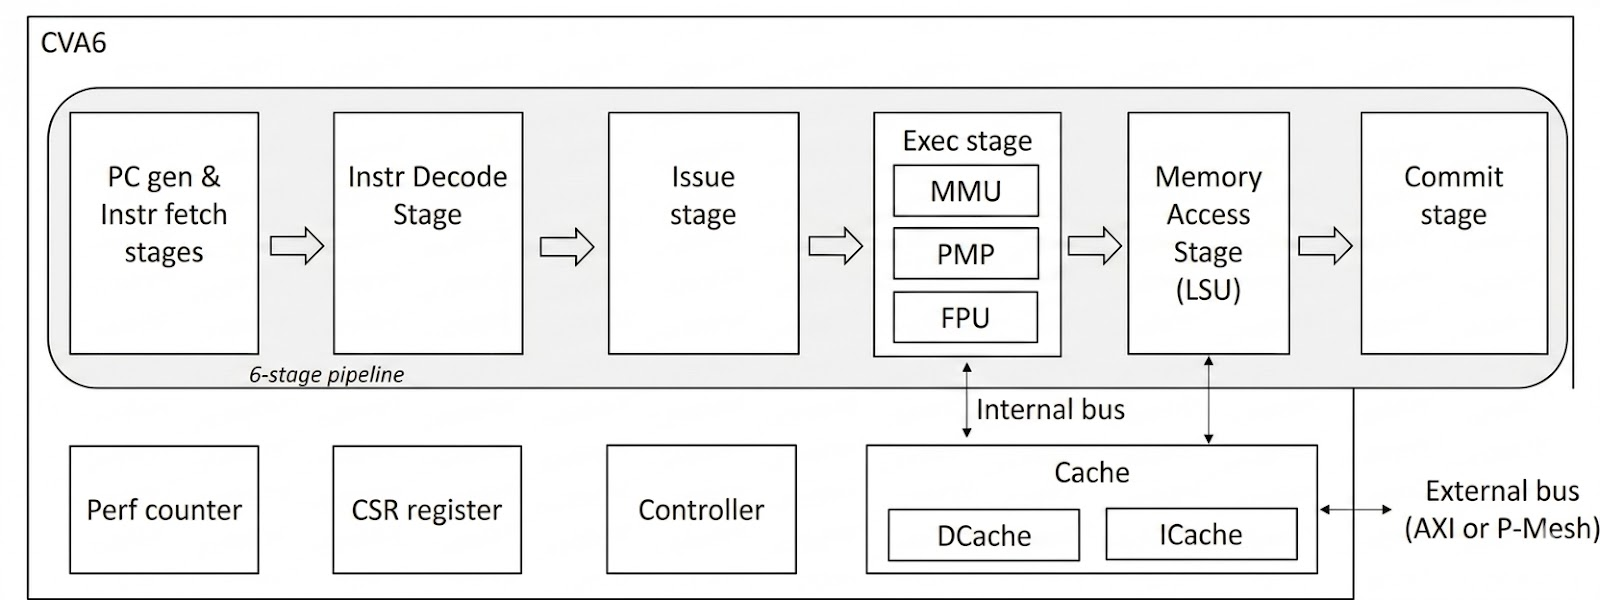
\includegraphics[angle=0,width=12cm]{./figures/cva6_block_complete1.jpg}
\label{fig:openhw}
\end{center}
\end{frame}
\begin{frame}[label={sec:orgf57656b}]{The CVA6 Core}
\framesubtitle{Benagil Team's Dual Core Version}
\begin{center}
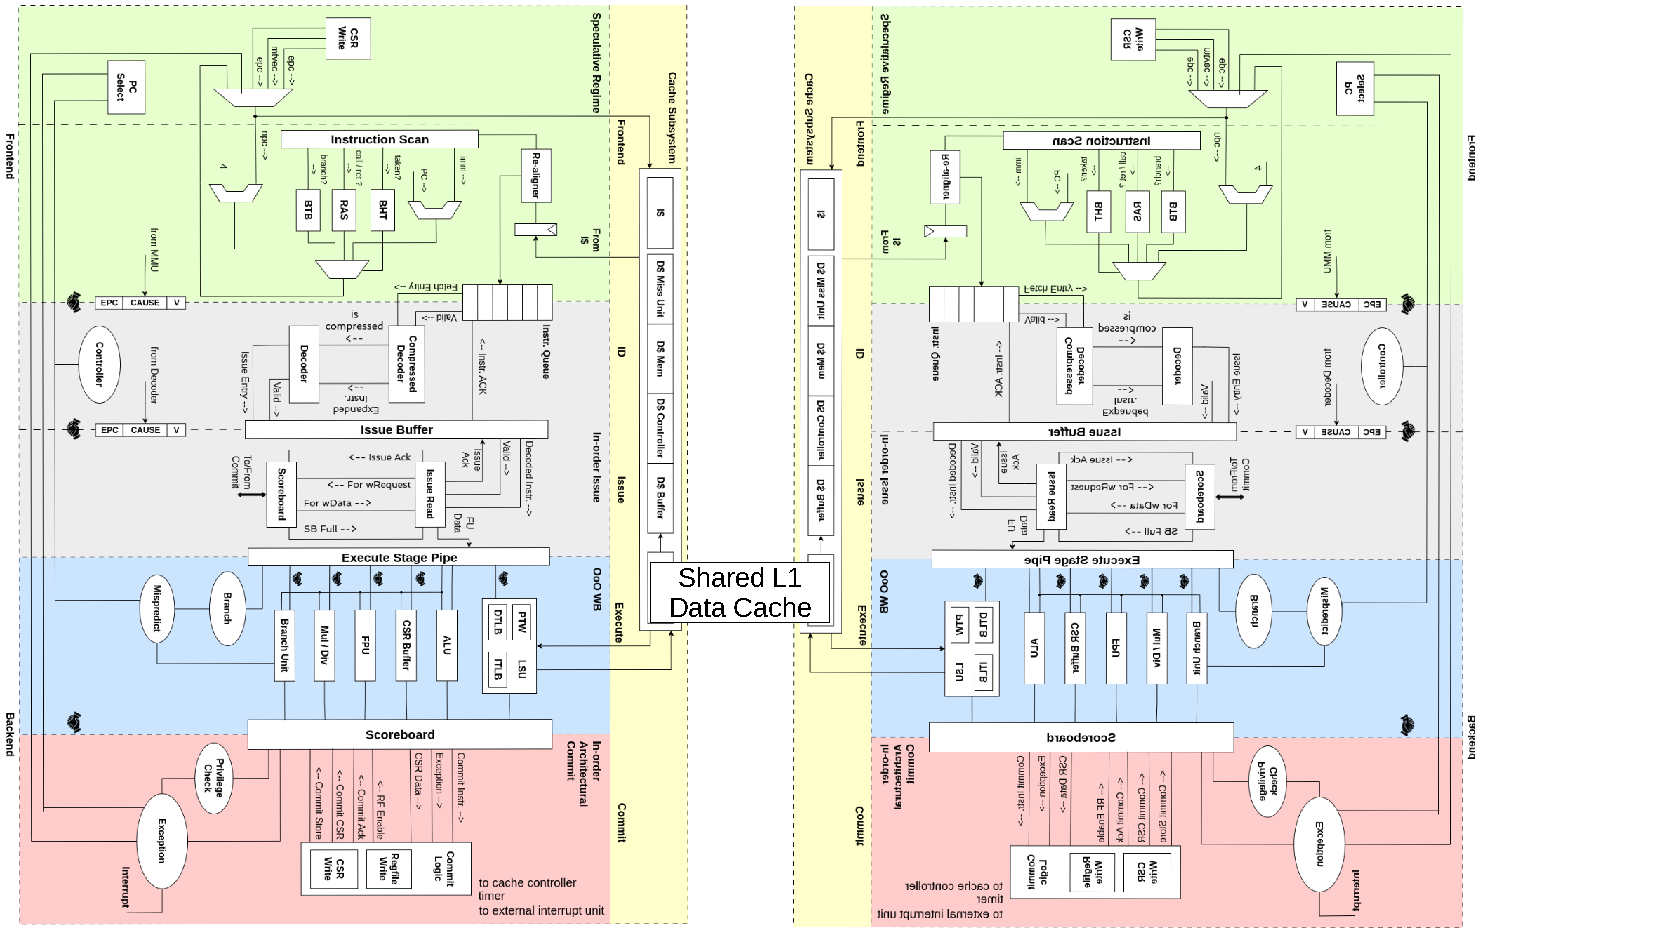
\includegraphics[trim=0 0 50 0, clip,width=\textwidth]{./figures/multicore_cva6.pdf}
\label{fig:dualcore}
\end{center}
\end{frame}
\begin{frame}[label={sec:org80e1fb9}]{Problem Statement}
\begin{alertblock}{Problem}
\small The dual-core system is limited by a 1-request-per-cycle bandwidth at the L1D cache.
\end{alertblock}
\begin{exampleblock}{Research Objectives}\label{sec:org3ff24f6}
\begin{itemize}
\item \small How does the sharing of functional units (starting with the FPU) between two CVA6 cores affect the trade-off between hardware area efficiency and multi-core performance?
\item \small How to measure it accurately.
\end{itemize}
\end{exampleblock}
\end{frame}
\begin{frame}[label={sec:org7f60640}]{Project Roadmap}
\begin{center}
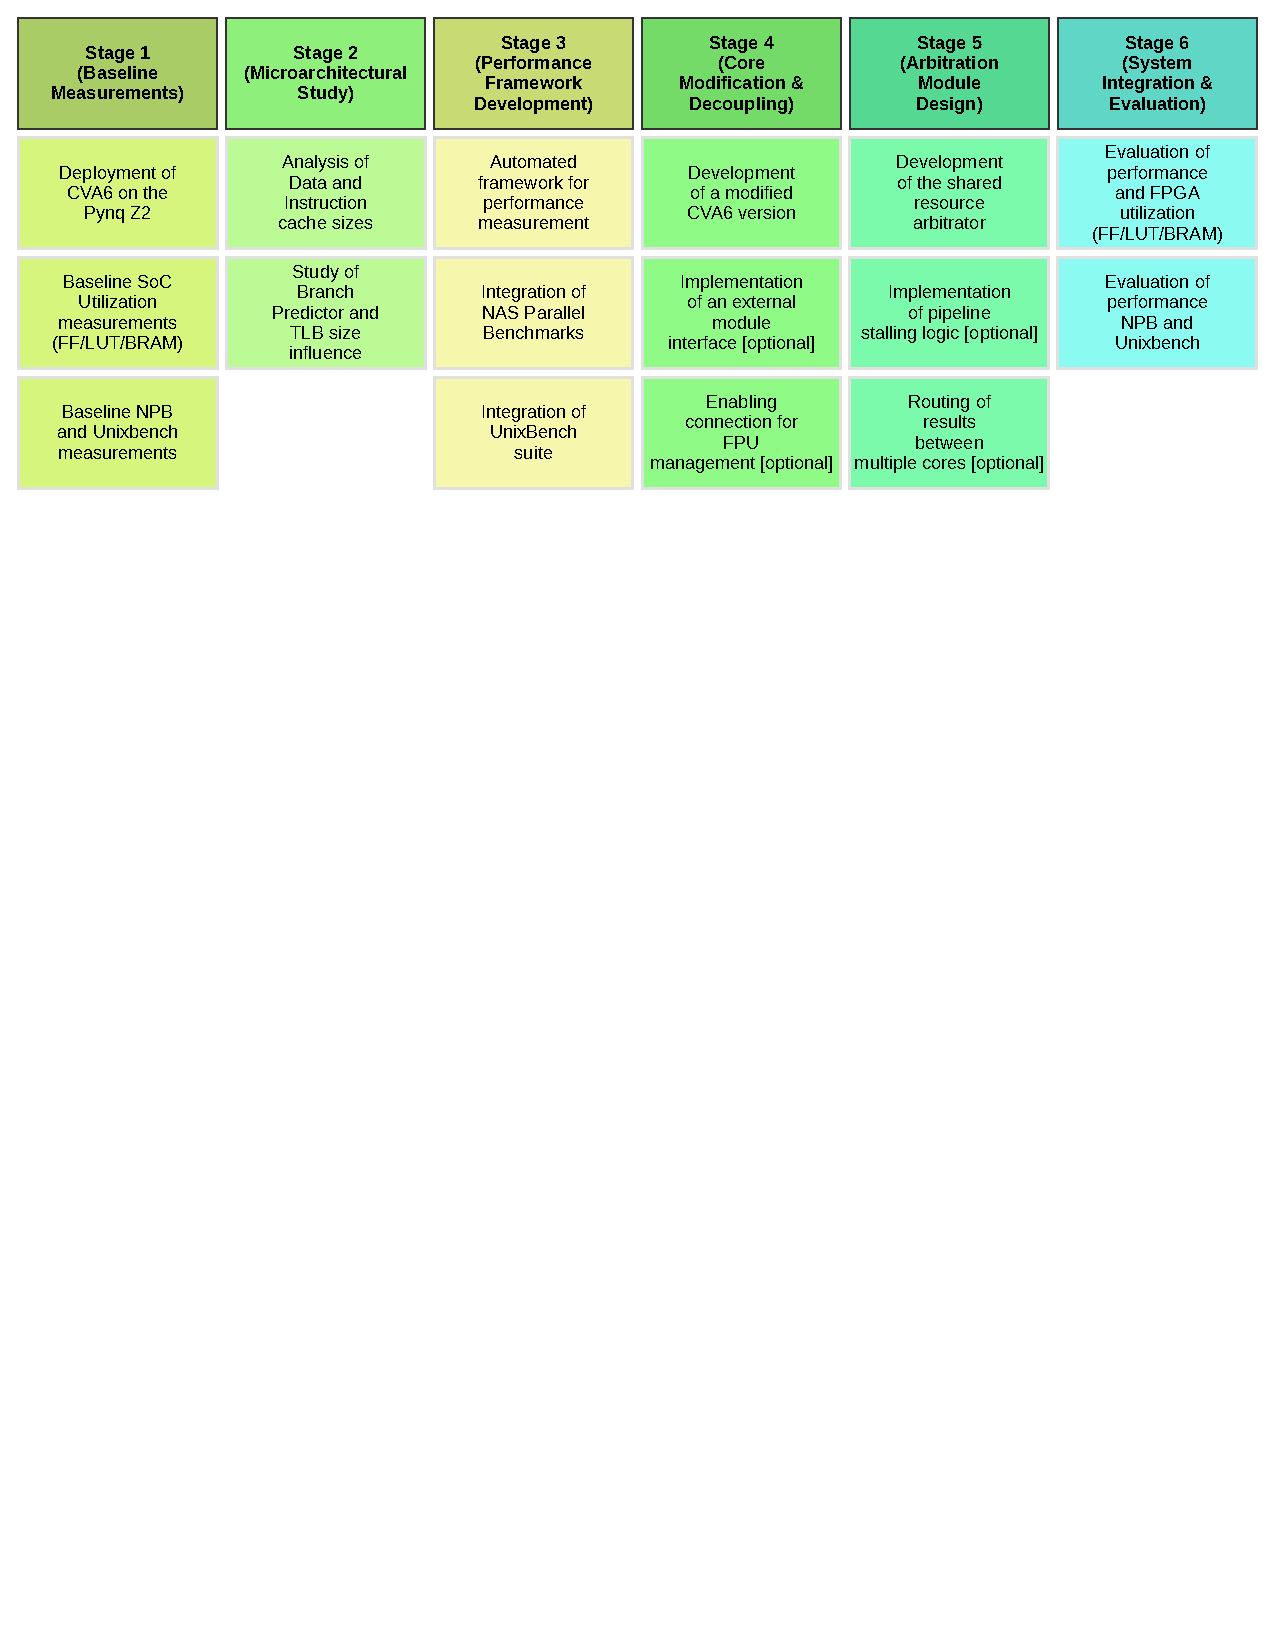
\includegraphics[trim=0 0 0 0, clip,width=\textwidth]{roadmap.pdf}
\label{fig:roadmap}
\end{center}
\end{frame}
\section{Performance and Resource Usage Measurement}
\label{sec:orgbe66f4b}
\begin{frame}[label={sec:orga4da74a}]{How do We Measure Performance?}
\framesubtitle{What do we measure?}
\small We evaluate performance using well-known workloads: UnixBench and the NAS Parallel Benchmarks (NPB). For each benchmark, we also measure instructions per cycle (\emph{IPC}).

\begin{equation}
\begin{split}
\(IPC = \frac{\text{Number of Instructions}}{\text{Number of cycles}}\)
\end{split}
\end{equation}

\begin{itemize}
\item \small Hardware performance counters. \emph{Single Core} available performance counters:
\begin{itemize}
\item Number of Instructions
\item Number of cycles
\end{itemize}

\item \small Benchmark scores:
\begin{itemize}
\item \small NPB: \alert{Mop/s (Millions of Operations per Second)}
\item \small Unixbench: \alert{Loops per second (lps), KB/sec, and operations per second}
\end{itemize}
\end{itemize}
\end{frame}
\begin{frame}[label={sec:org140a0ba}]{How do We Measure Performance and Resource Usage?}
\framesubtitle{Experimental Setup}

\begin{figure}[!htb]
\centering
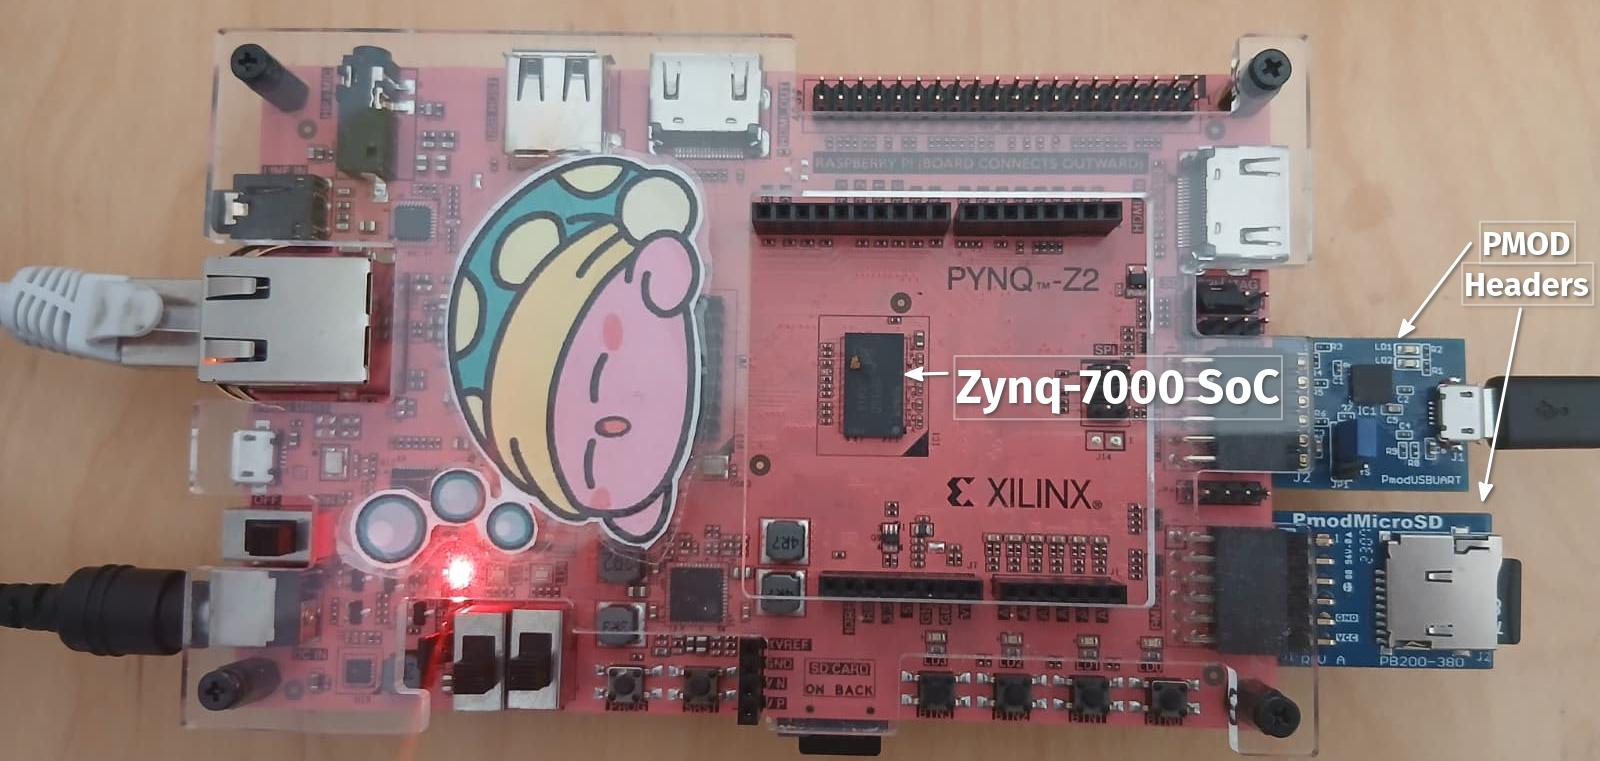
\includegraphics[angle=0,width=11.0cm]{./figures/pynq.jpeg}
\caption{\label{fig:pynq}CVA6 \emph{Single Core} deployment on a PYNQ-Z2 FPGA with PMod Modules}
\end{figure}
\end{frame}
\begin{frame}[label={sec:org8918803}]{How do We Measure Resource Usage?}
\begin{columns}
\begin{column}{0.6\columnwidth}
\begin{figure}[!htb]
\centering
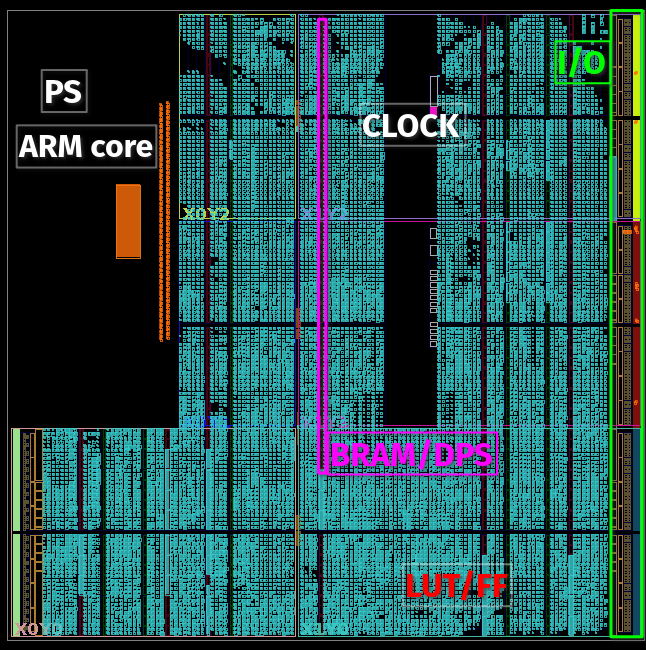
\includegraphics[angle=0,width=6.3cm]{./figures/PL_block.png}
\caption{\label{fig:pynq}Zynq-7000 SoC}
\end{figure}
\end{column}
\begin{column}{0.4\columnwidth}
\footnotesize The SoC (System on a chip) is mapped onto the FPGA’s programmable logic, utilizing the following hardware resources to implement the CVA6 design:

\begin{itemize}
\item \footnotesize Look Up Tables (\alert{LUT}) for combinatorial logic.
\item \footnotesize Flip Flops (\alert{FF}) for state storage
\item \footnotesize Block Random Access Memory (\alert{BRAM}) for fast on-chip memory
\item \footnotesize Digital Signal Processor (\alert{DSP}) for high-performance math calculations
\end{itemize}
\end{column}
\end{columns}
\end{frame}
\begin{frame}[label={sec:org64148f6}]{How do We Measure Resource Usage?}
\framesubtitle{Initial LUT Usage Measurement}
\begin{center}
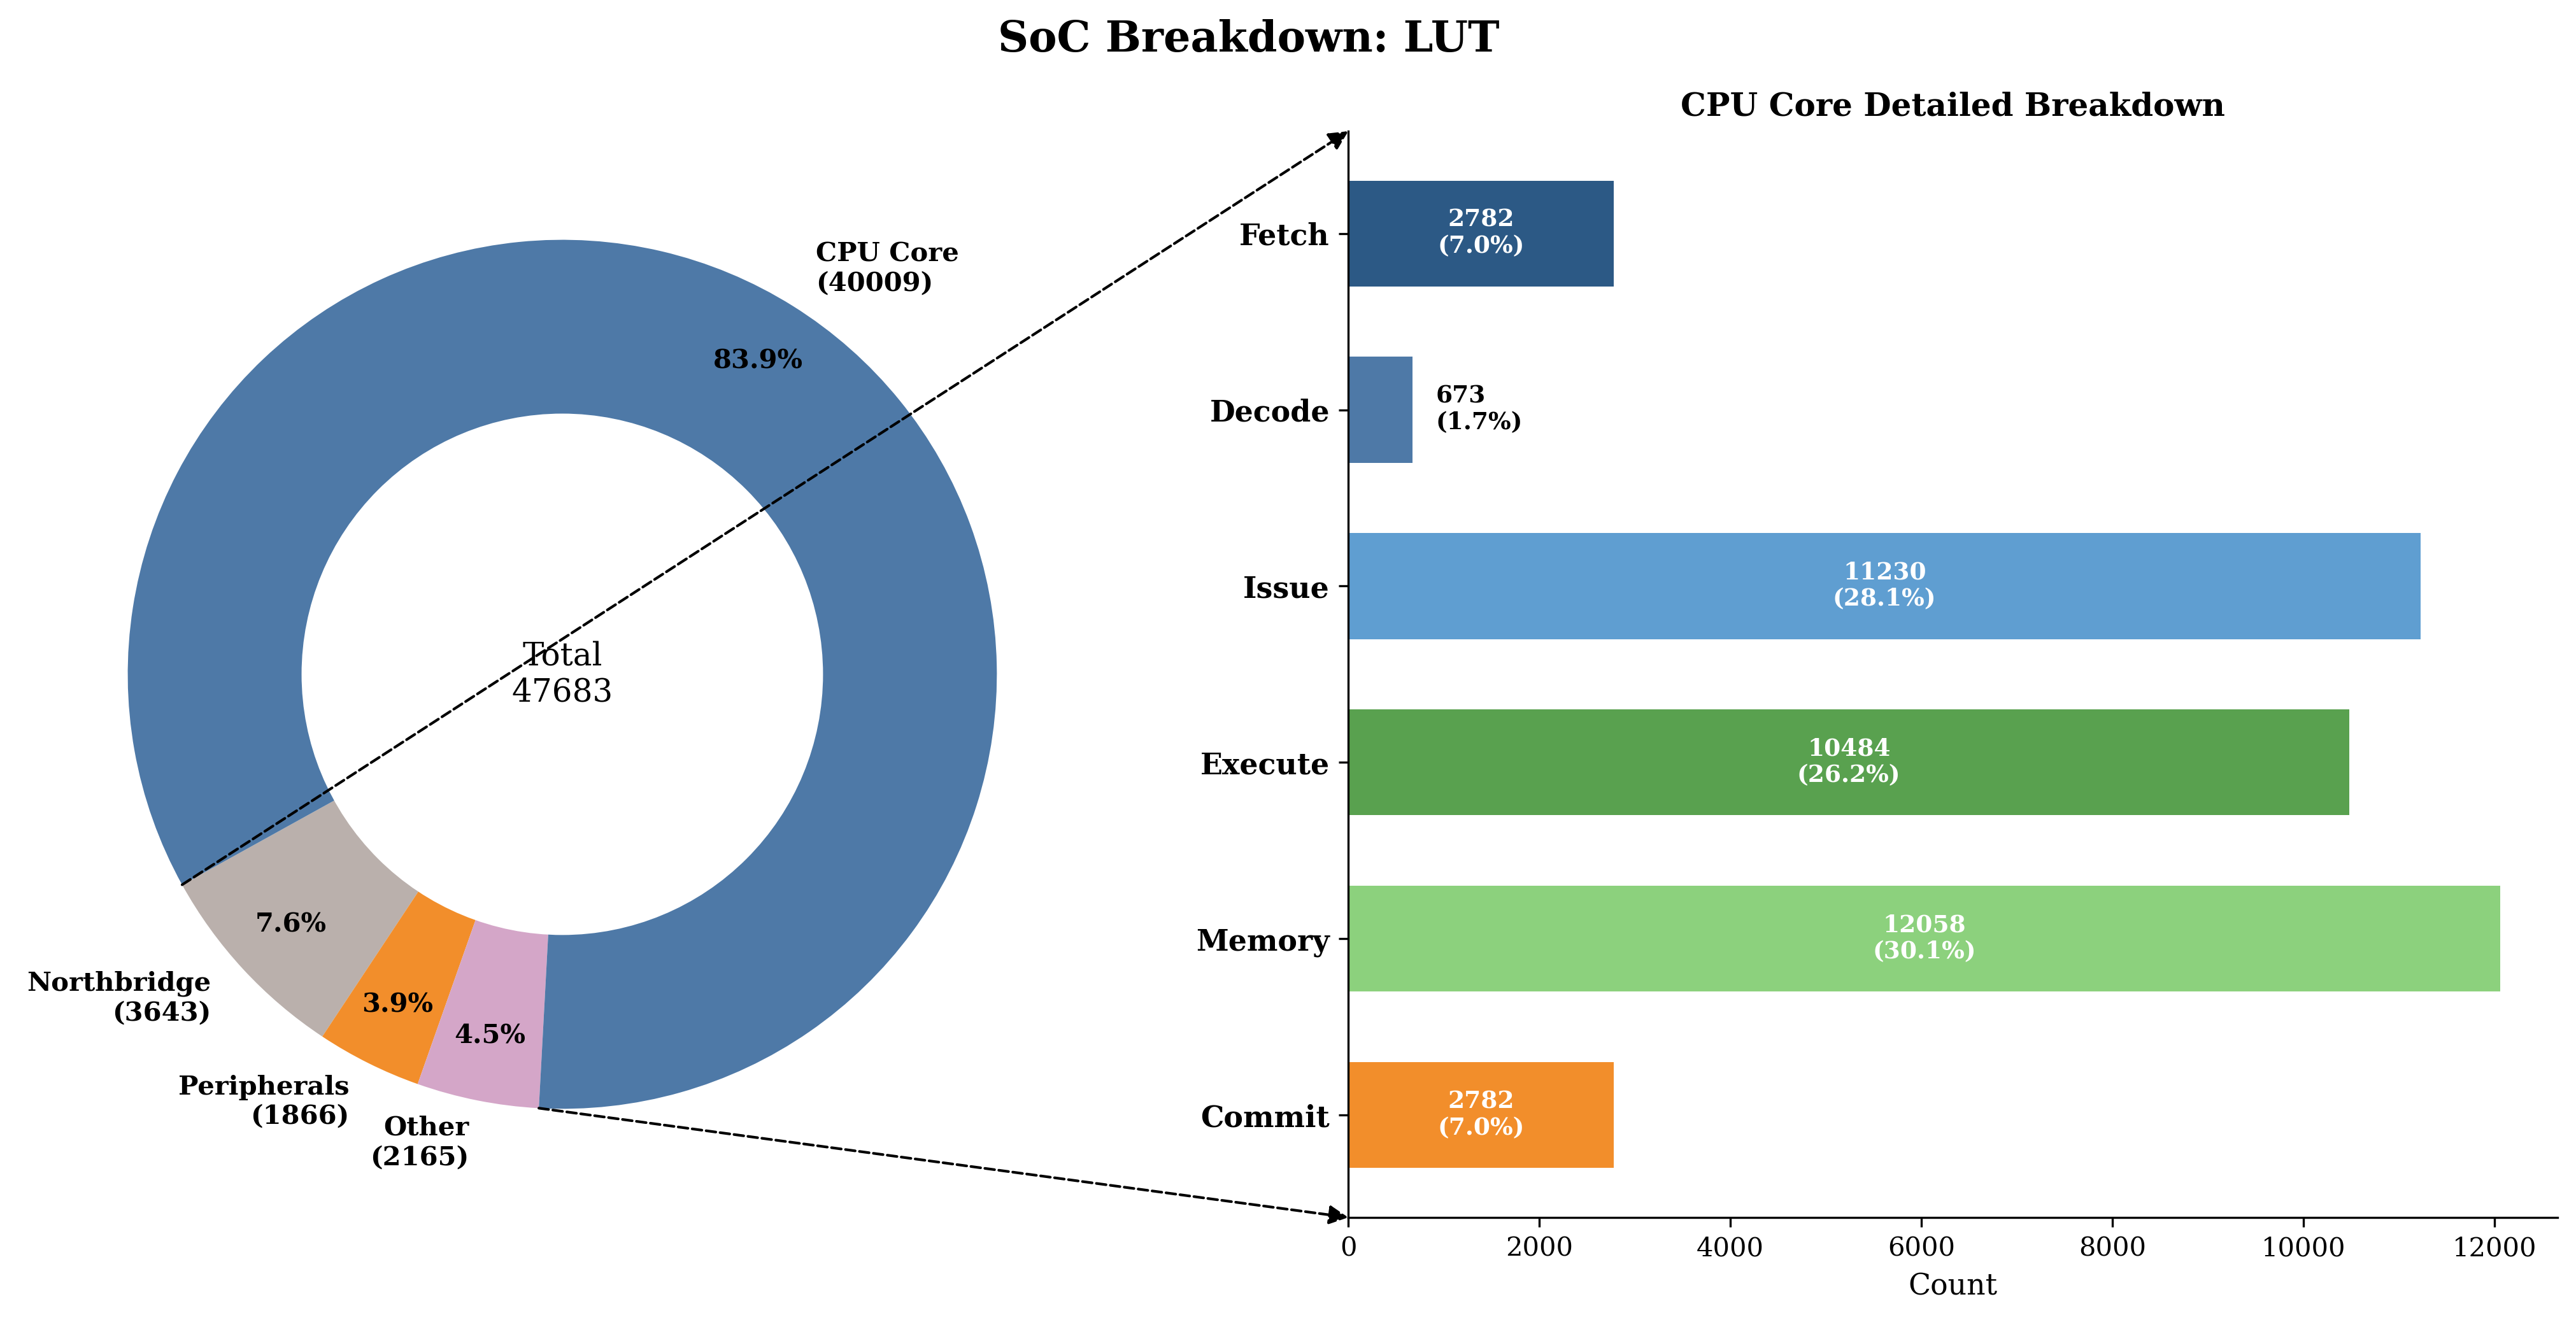
\includegraphics[angle=0,width=12.0cm]{./figures/soc_breakdown_bar_pie_h_final_LUT.png}
\label{fig:base_lut}
\end{center}
\end{frame}
\begin{frame}[label={sec:org59663b9}]{How do We Measure Resource Usage?}
\framesubtitle{Initial FF Usage Measurement}
\begin{center}
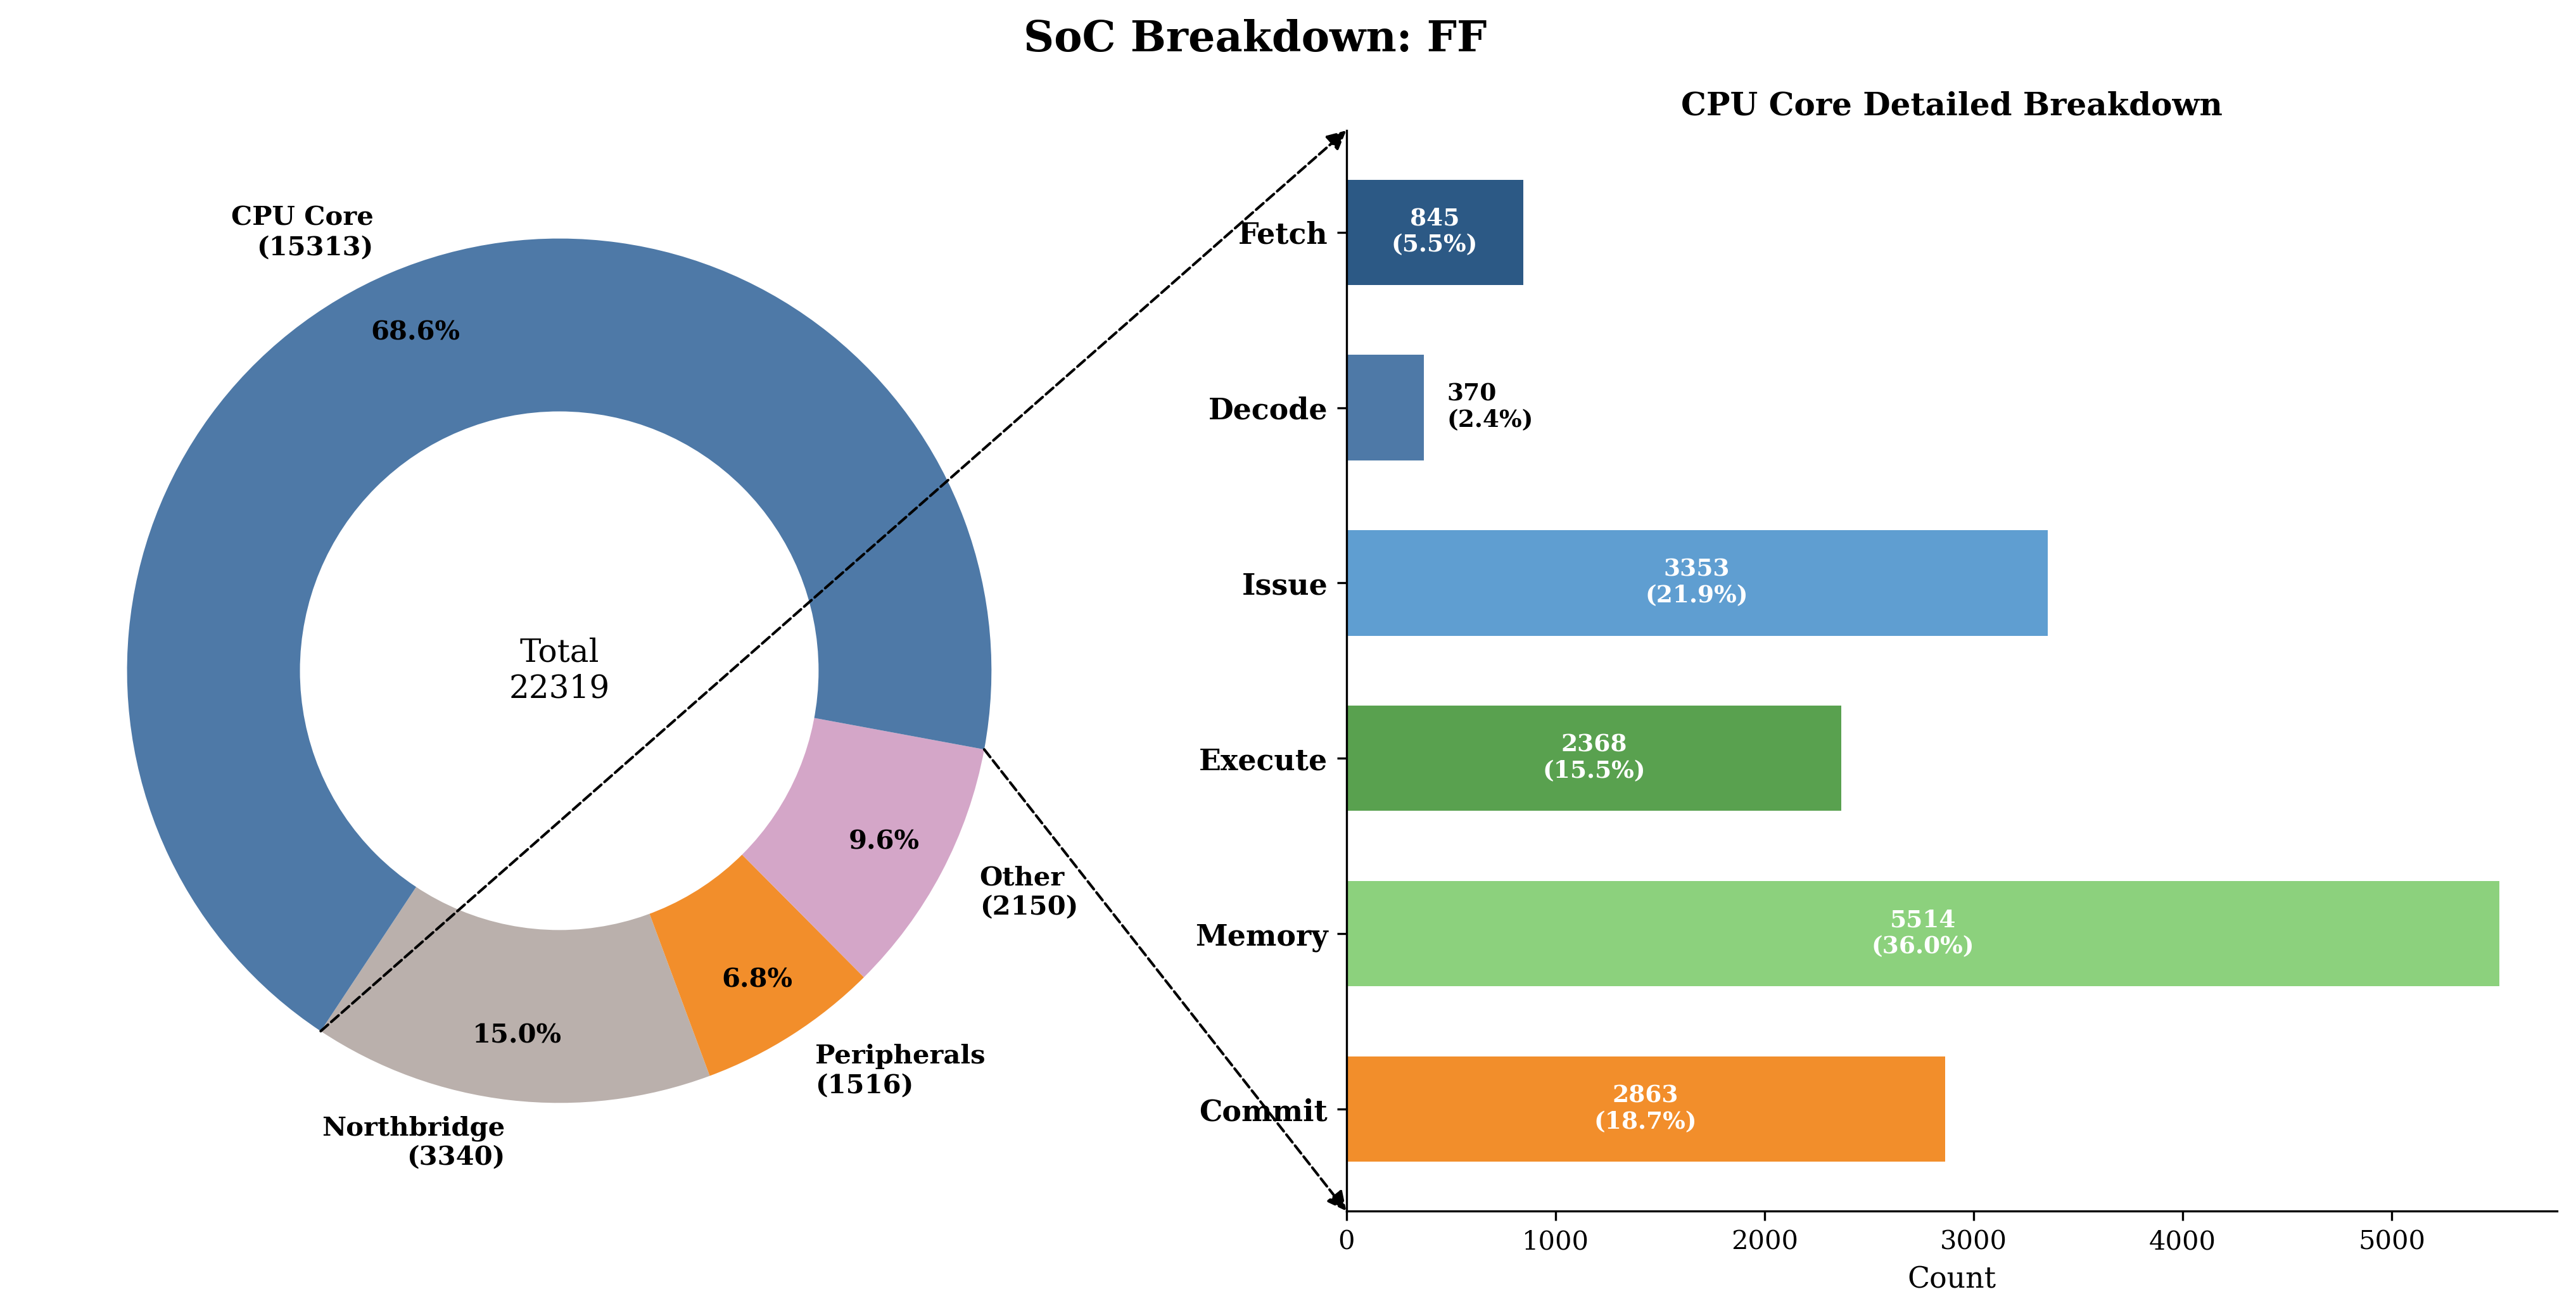
\includegraphics[angle=0,width=12.0cm]{./figures/soc_breakdown_bar_pie_h_final_FF.png}
\label{fig:base_ff}
\end{center}
\end{frame}
\begin{frame}[label={sec:org1e333fc}]{How do We Measure Resource Usage?}
\framesubtitle{Initial BRAM Usage Measurement}
\begin{center}
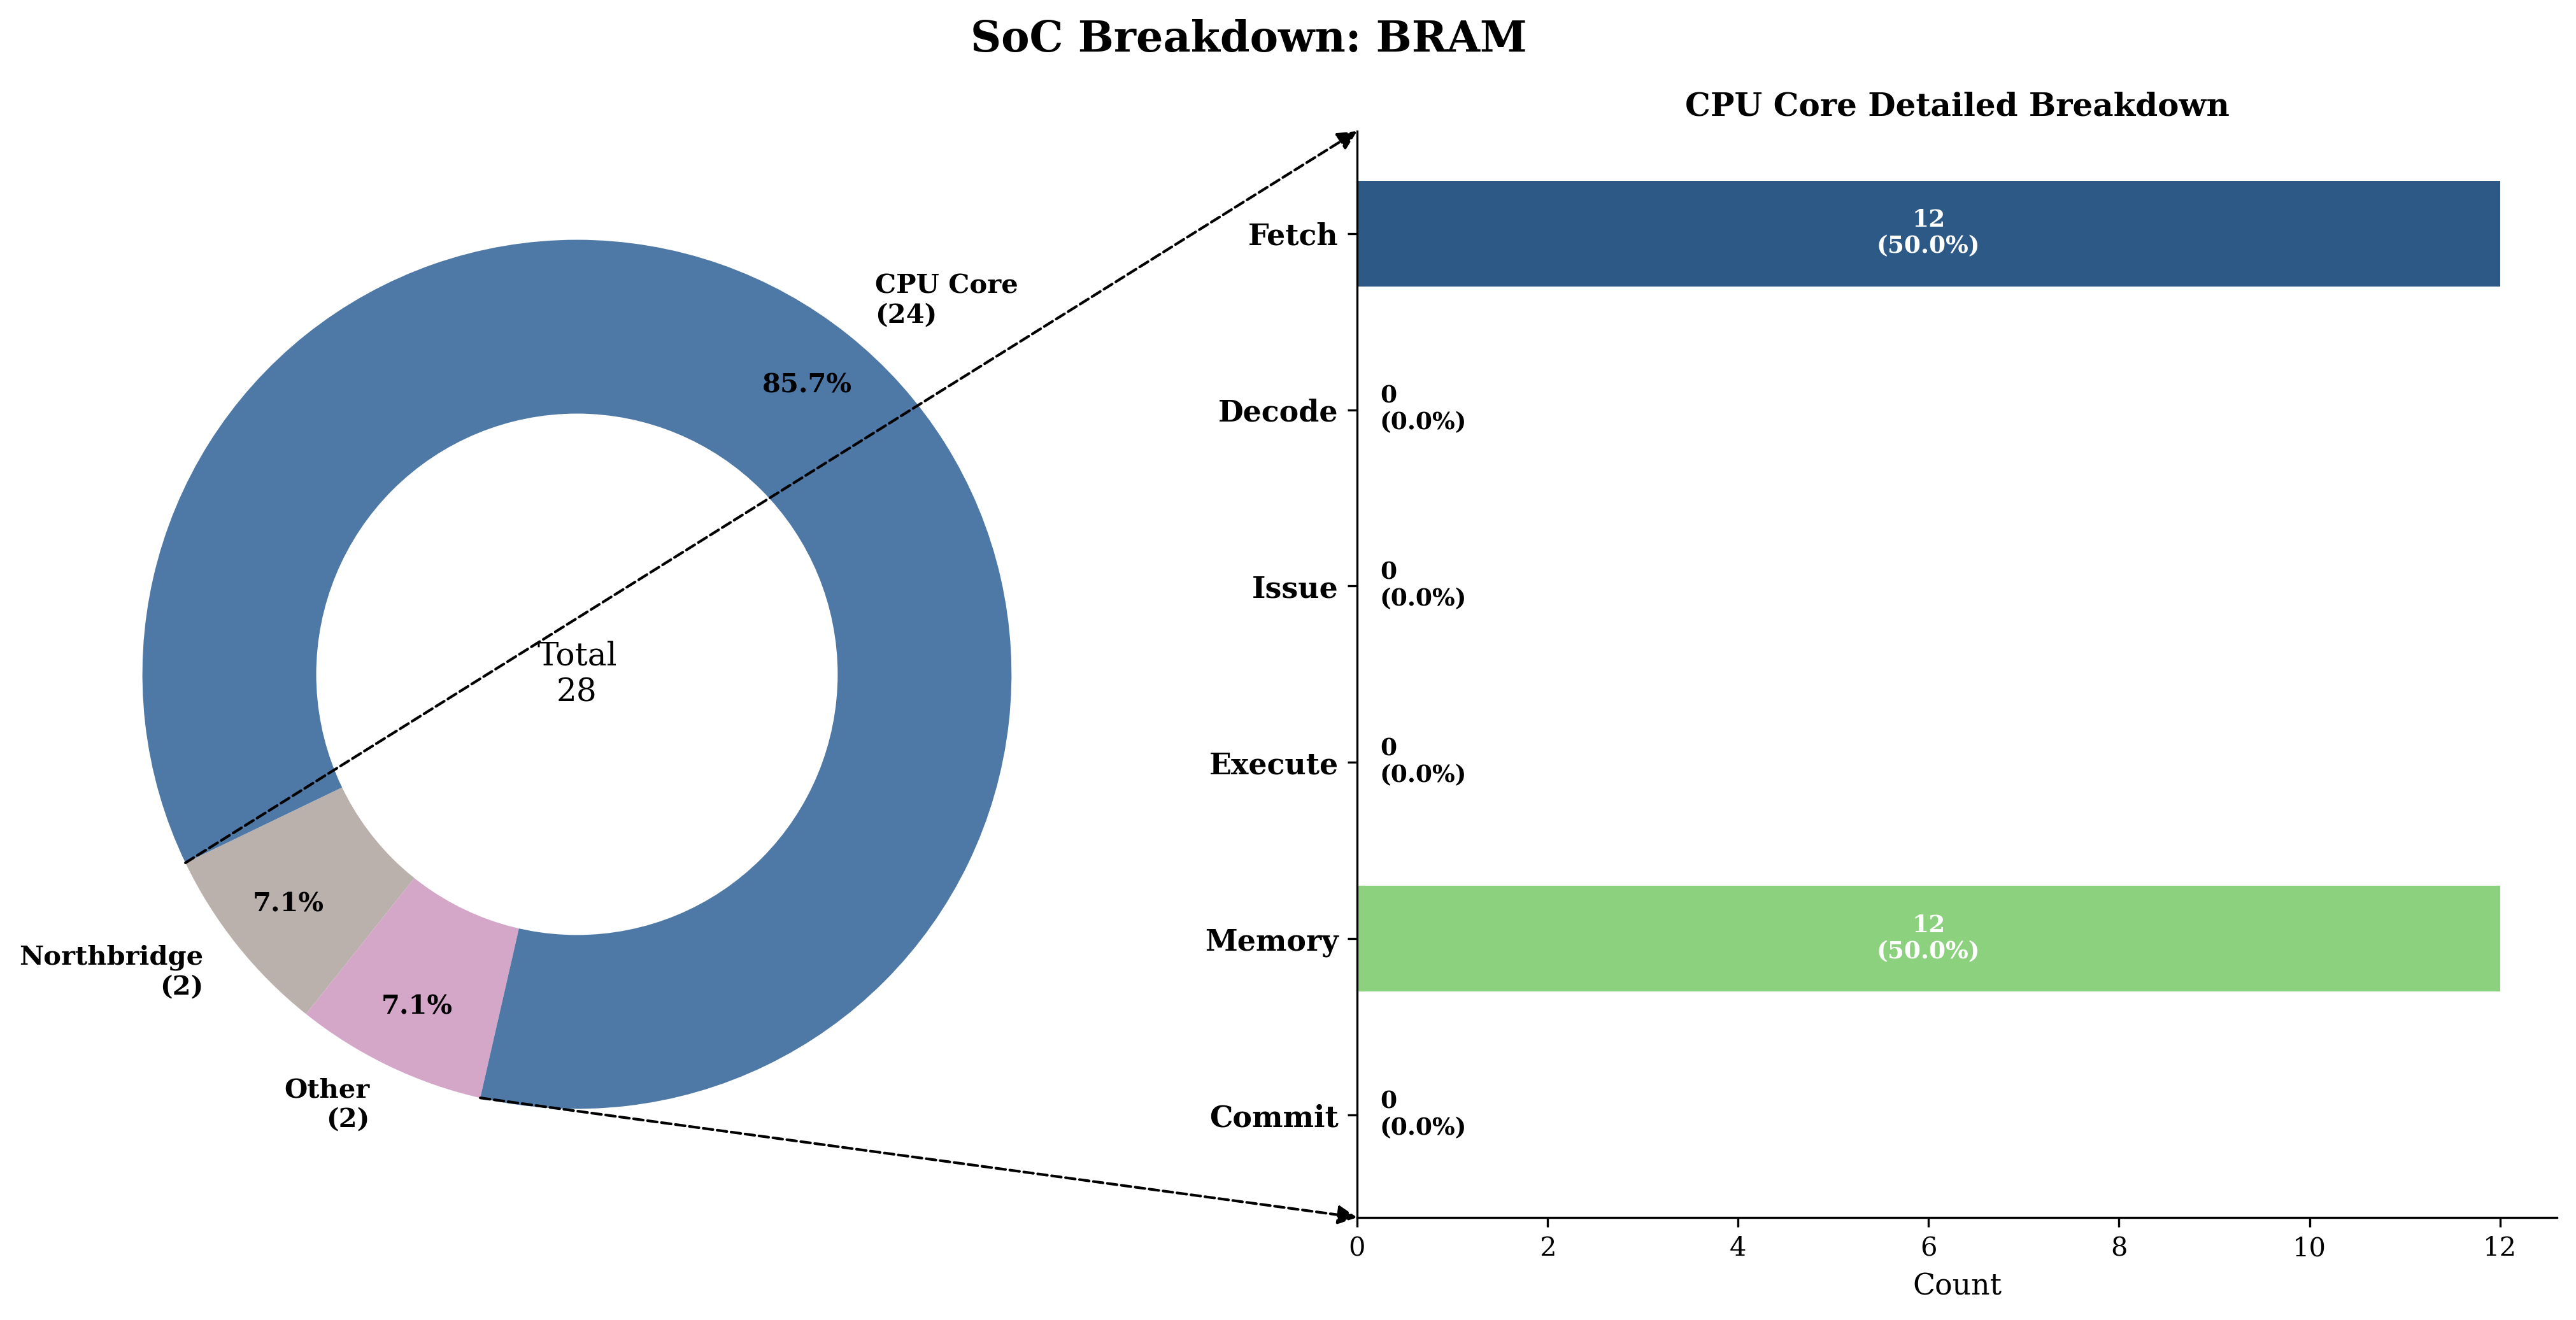
\includegraphics[angle=0,width=12.0cm]{./figures/soc_breakdown_bar_pie_h_final_BRAM.png}
\label{fig:base_bram}
\end{center}
\end{frame}
\begin{frame}[label={sec:org96c26a1}]{How do We Measure Resource Usage?}
\framesubtitle{Initial DSP Usage Measurement}
\begin{center}
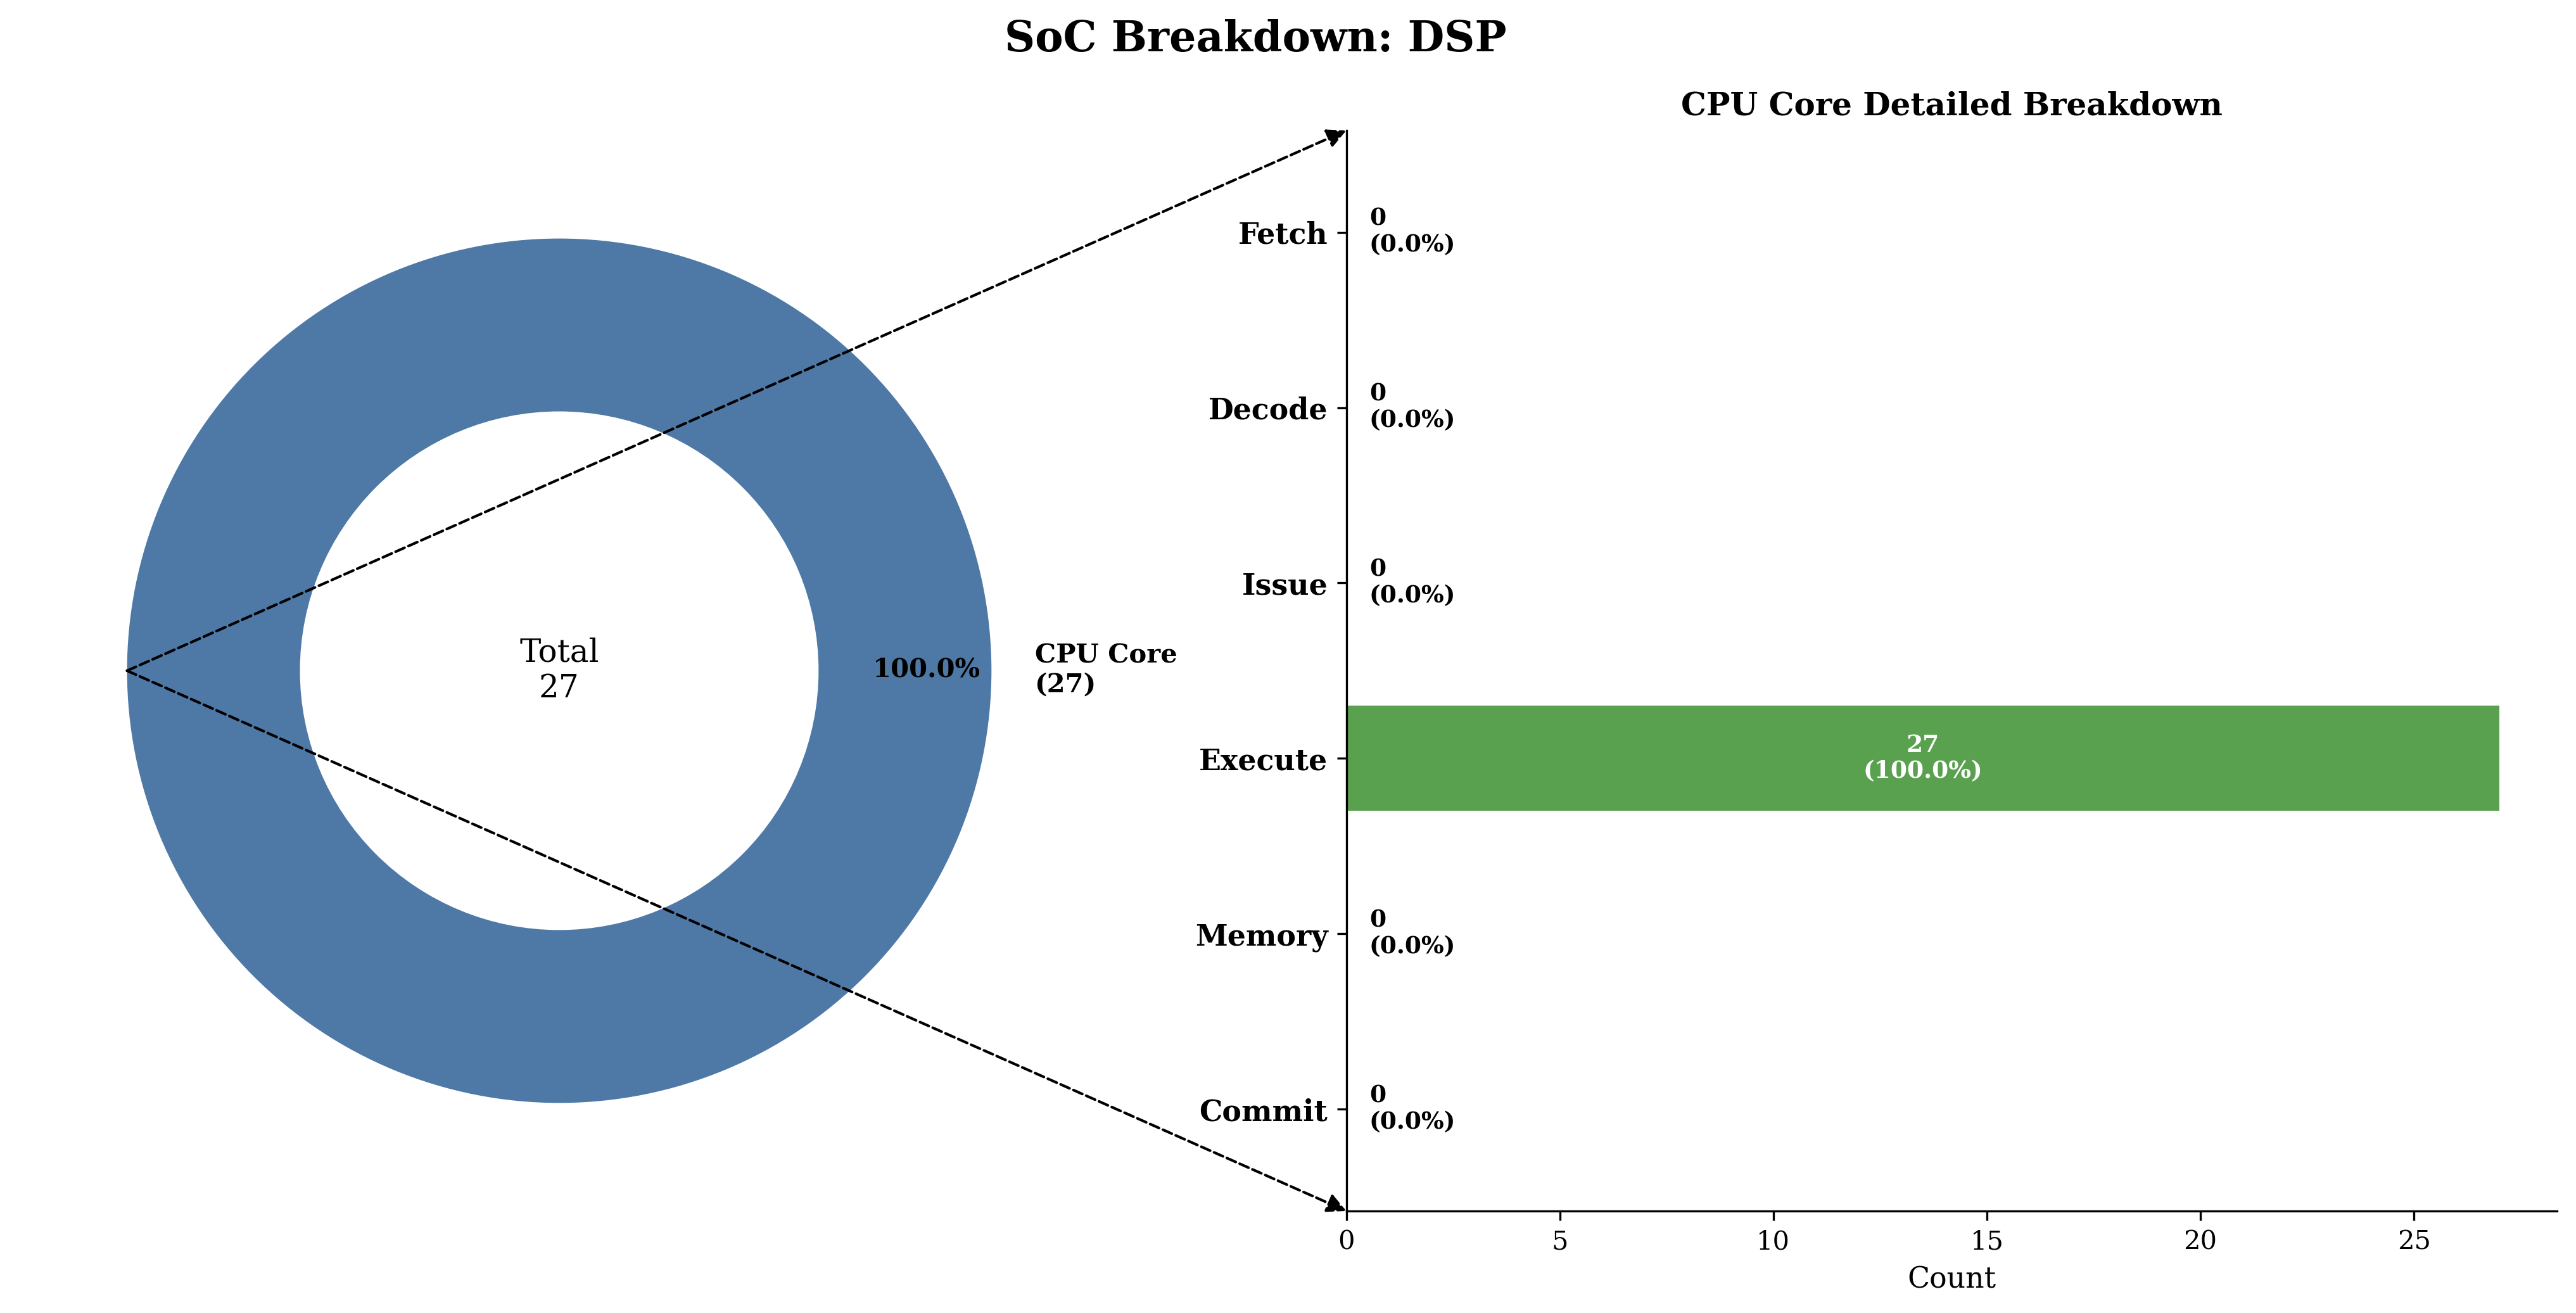
\includegraphics[angle=0,width=12.0cm]{./figures/soc_breakdown_bar_pie_h_final_DSP.png}
\label{fig:base_dsp}
\end{center}
\end{frame}
\section{Experiments}
\label{sec:org822c091}
\begin{frame}[label={sec:orgcec8fc3}]{Baseline Architecture}
To study the effects of the micro-architectural parameters the following baseline parameters were used.
\begin{table}[htbp]
\label{tab:baseline_parameters}
\centering
\begin{tabular}{lll}
\hline
\alert{Parameter} & \alert{Size} & \alert{CVA6 Stage}\\
\hline
Data Cache & \(4096[bytes]\) & Memory\\
\hline
Data Cache Associativity & 4 & Memory\\
\hline
Data Cache Line Width & 128 & Memory\\
\hline
Instruction Cache & \(4096[bytes]\) & Fetch\\
\hline
Instruction Cache Associativity & 4 & Fetch\\
\hline
Instruction Cache Line Width & 128 & Fetch\\
\hline
Branch Target Buffer (BTB) Entries & 16 & Fetch\\
\hline
Branch History Table (BHT) Entries & 16 & Fetch\\
\hline
Retirement Width of the CPU & 2 & Commit\\
\hline
\end{tabular}
\end{table}
\end{frame}
\begin{frame}[label={sec:org9e3504d}]{Parameter Sweeps}
And the following parameters sweeps were proposed to study their effect on performance and resource utilization.

\begin{table}[htbp]
\label{tab:baseline_parameters}
\centering
\begin{tabular}{lll}
\hline
\alert{Sweep} & \alert{Range} & \alert{CVA6 Stage}\\
\hline
Data Cache & \(128[bytes]\to256k[bytes]\) & Memory\\
\hline
Data / Instruction & \(1\to16\) & Memory / Fetch\\
Cache Associativity &  & \\
\hline
Instruction Cache & \(2k[bytes]\to256k[bytes]\) & Fetch\\
\hline
BTB Entries & \(8\to32k\) & Fetch\\
\hline
BHT Entries & \(16\to16k\) & Fetch\\
\hline
Retirement Width & \(2\to1\) & Commit\\
of the CPU &  & \\
\hline
\end{tabular}
\end{table}
\end{frame}
\begin{frame}[label={sec:org8937449}]{Automated Benchmarking Framework}
To automate the design space exploration we developed a framework which uses the ARM core and the CVA6 flashed into the FPGA.
\begin{center}
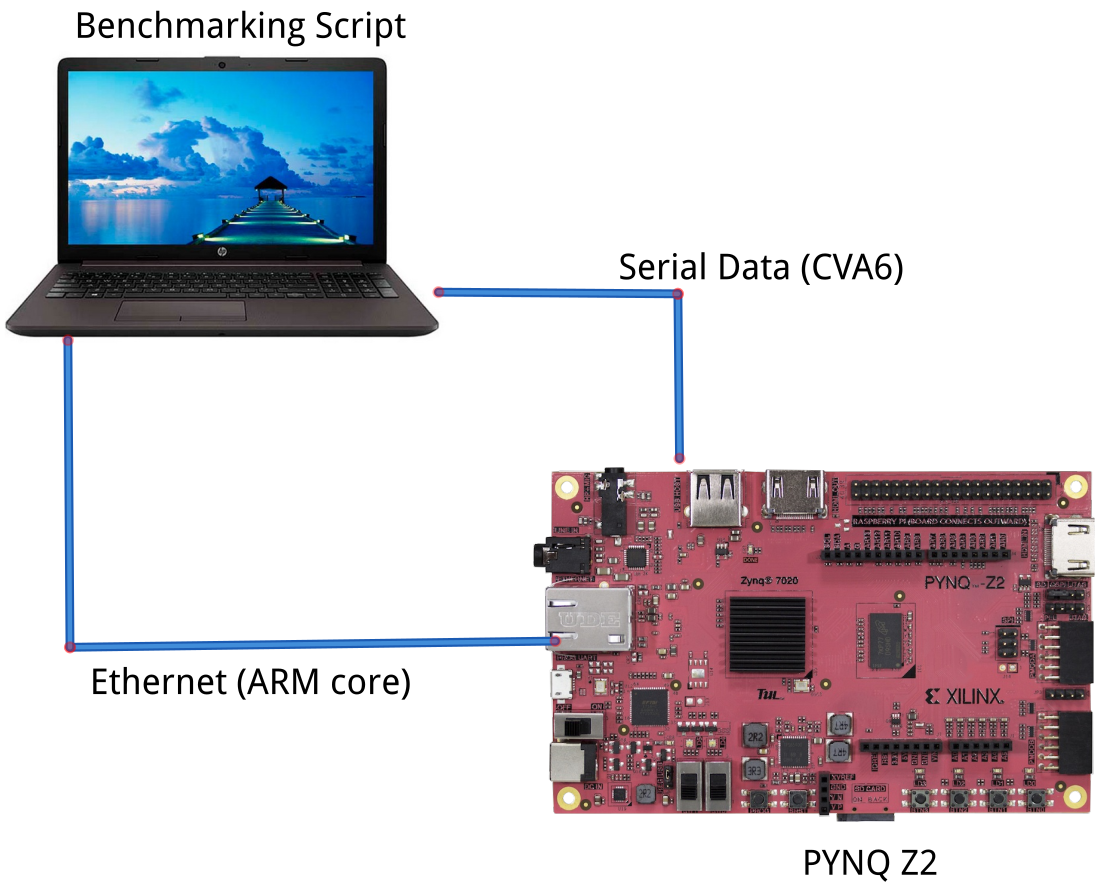
\includegraphics[angle=0,width=7.0cm]{./figures/bench.png}
\label{fig:base_dsp}
\end{center}
\end{frame}
\section{Results}
\label{sec:orgfa7efe1}
\begin{frame}[label={sec:org5a85932}]{Performance Dynamics}
\begin{center}
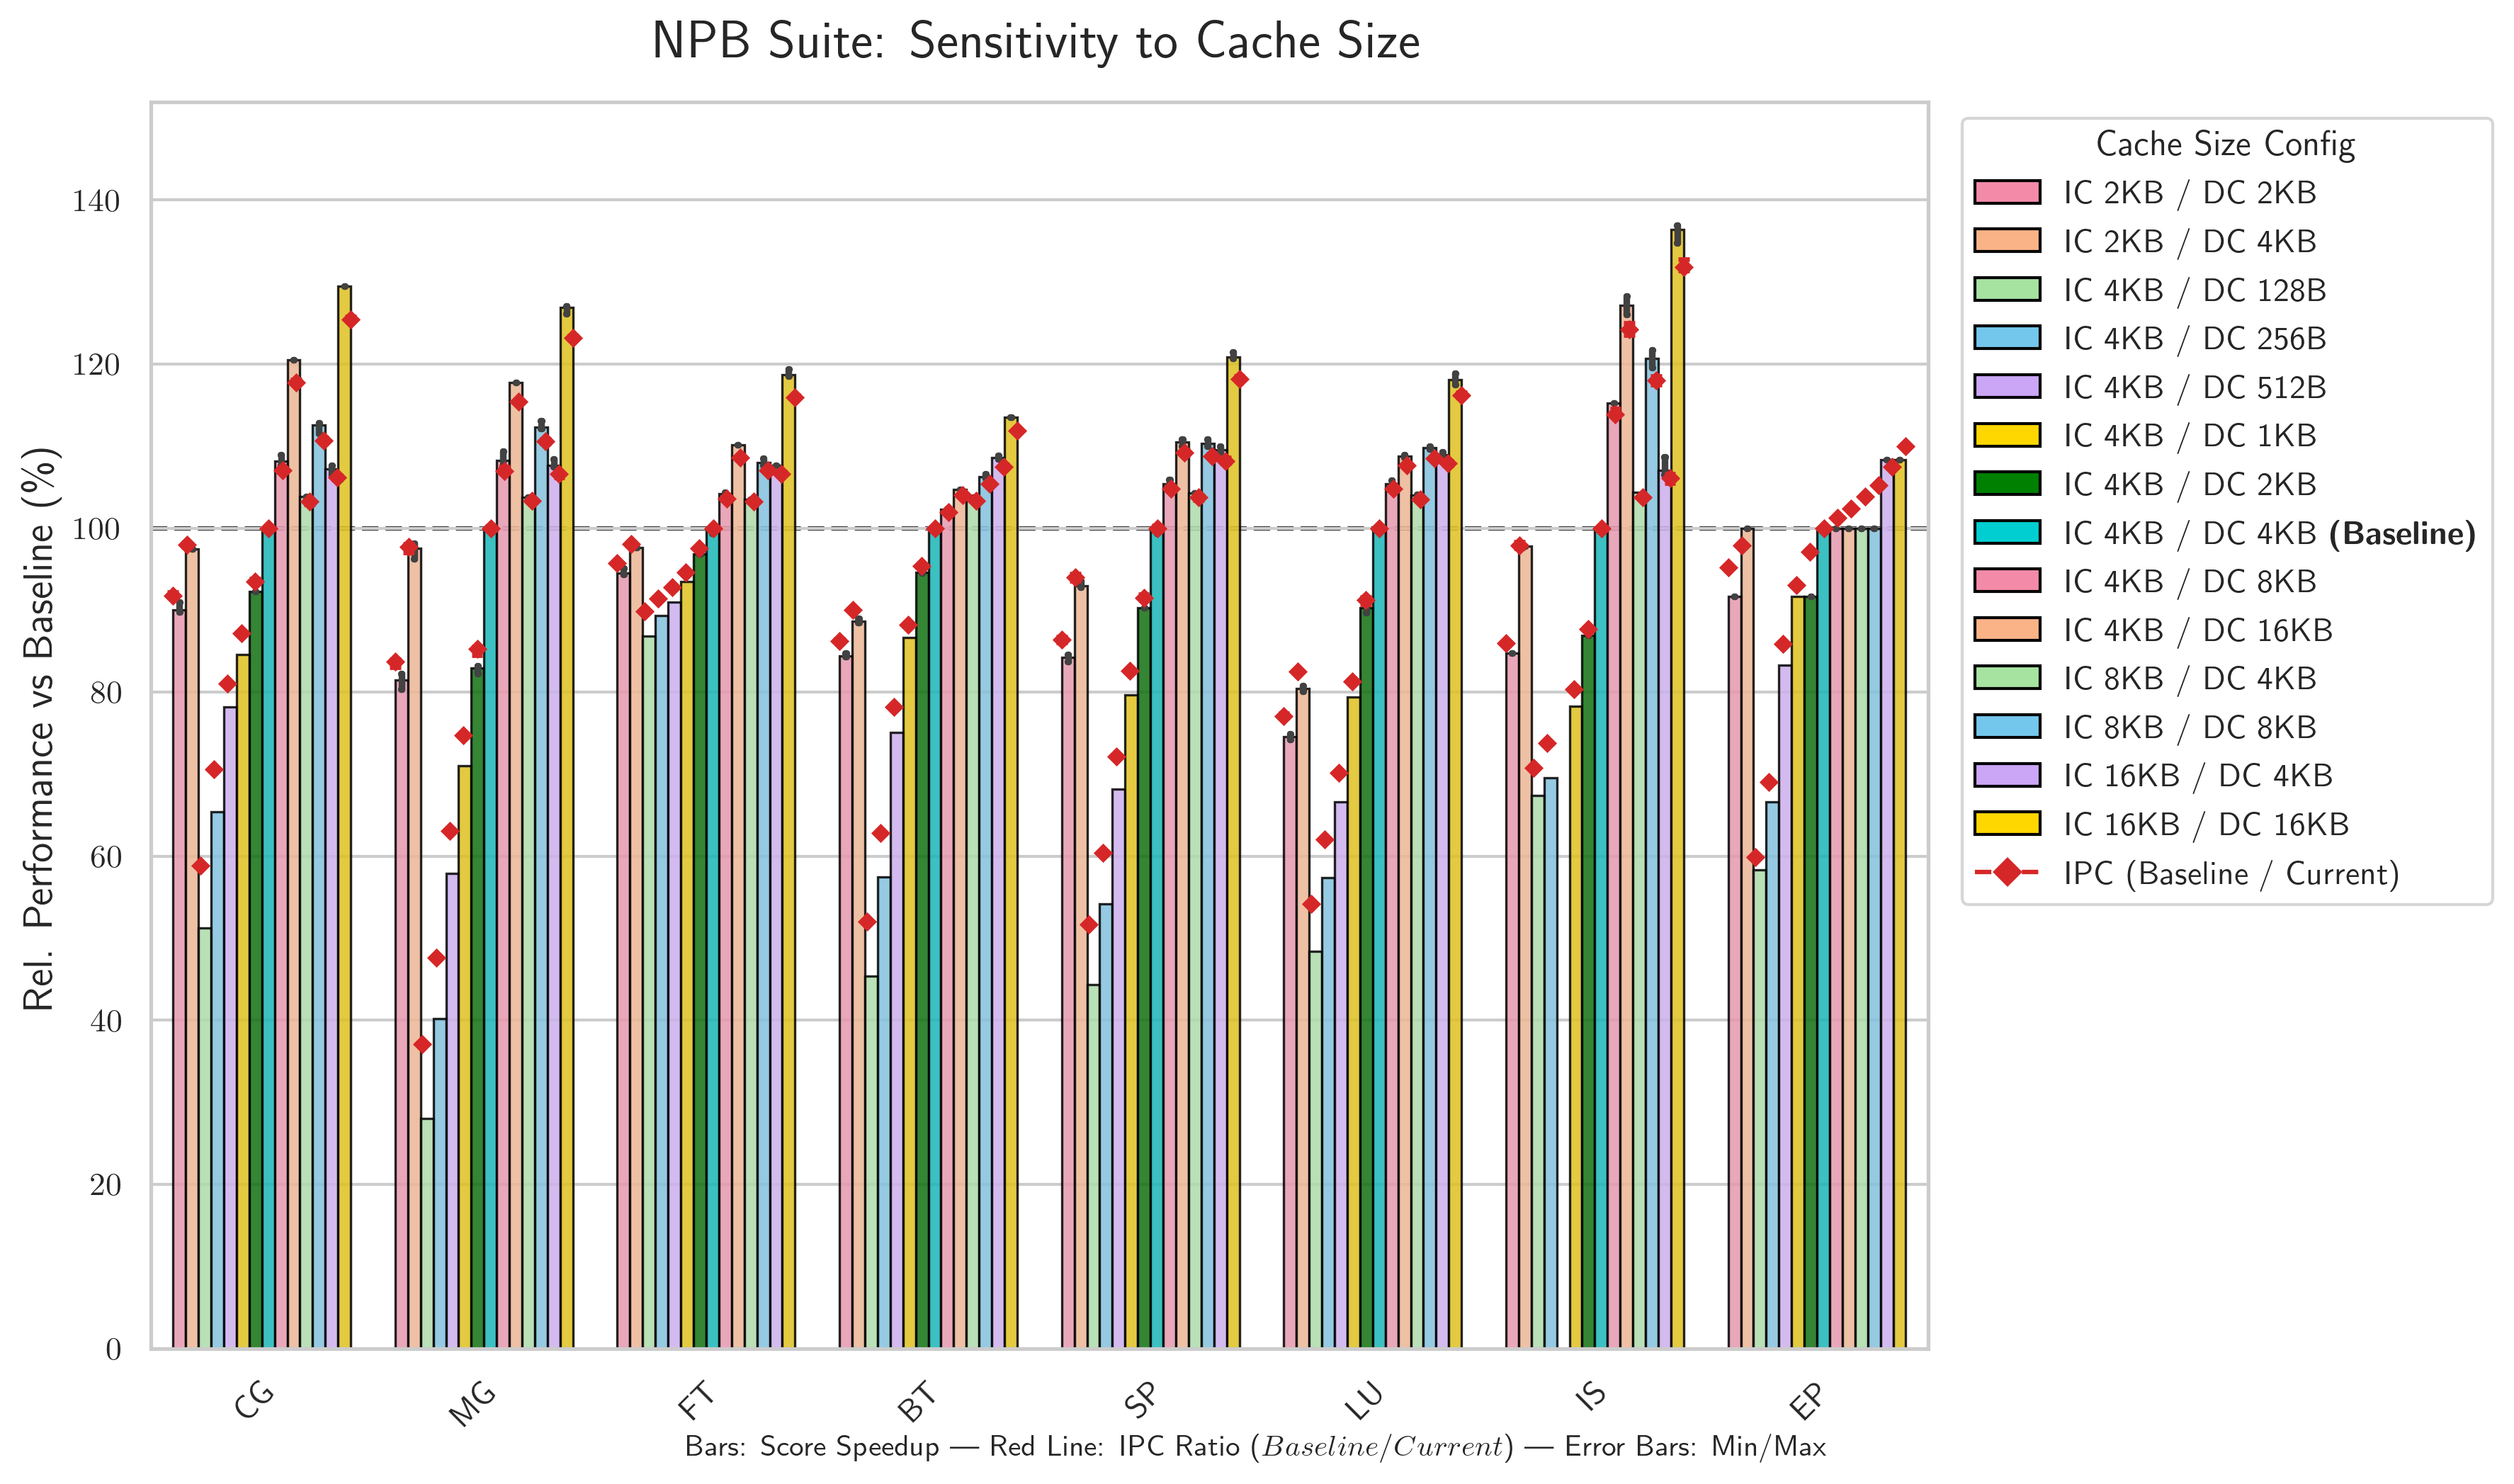
\includegraphics[angle=0,width=12.0cm]{./figures/cache_size_npb.png}
\label{fig:base_bram}
\end{center}
\end{frame}
\begin{frame}[label={sec:orga376672}]{Performance Dynamics}
\begin{center}
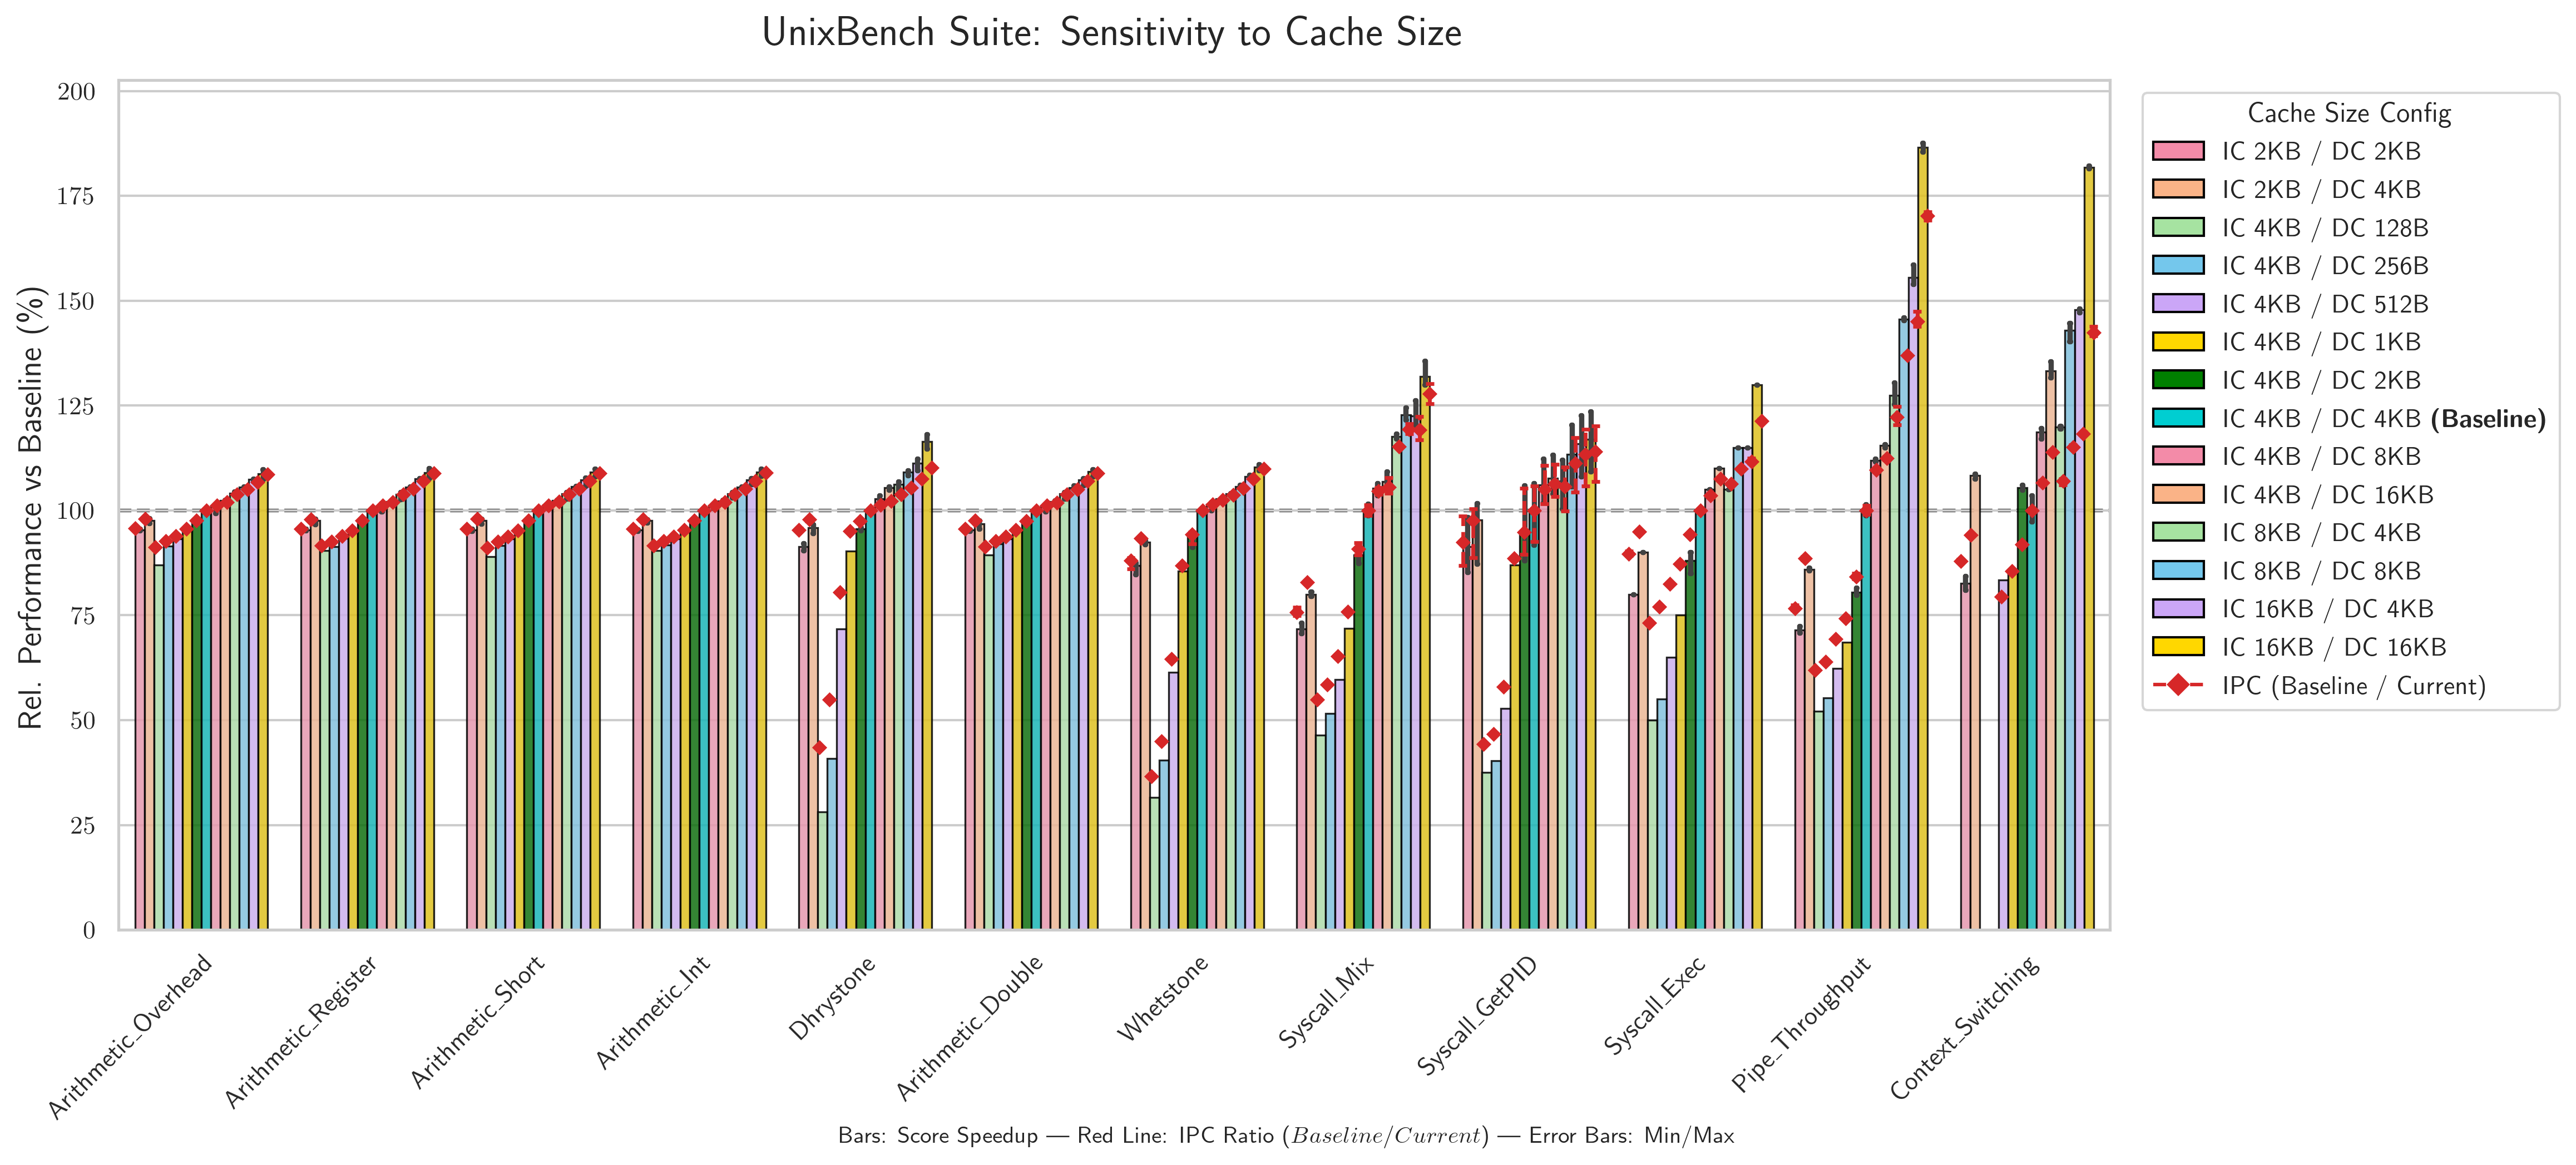
\includegraphics[angle=0,width=12.0cm]{./figures/cache_size_unixbench.png}
\label{fig:base_bram}
\end{center}
\end{frame}
\begin{frame}[label={sec:org278df0f}]{Resource Usage Dynamics}
\begin{center}
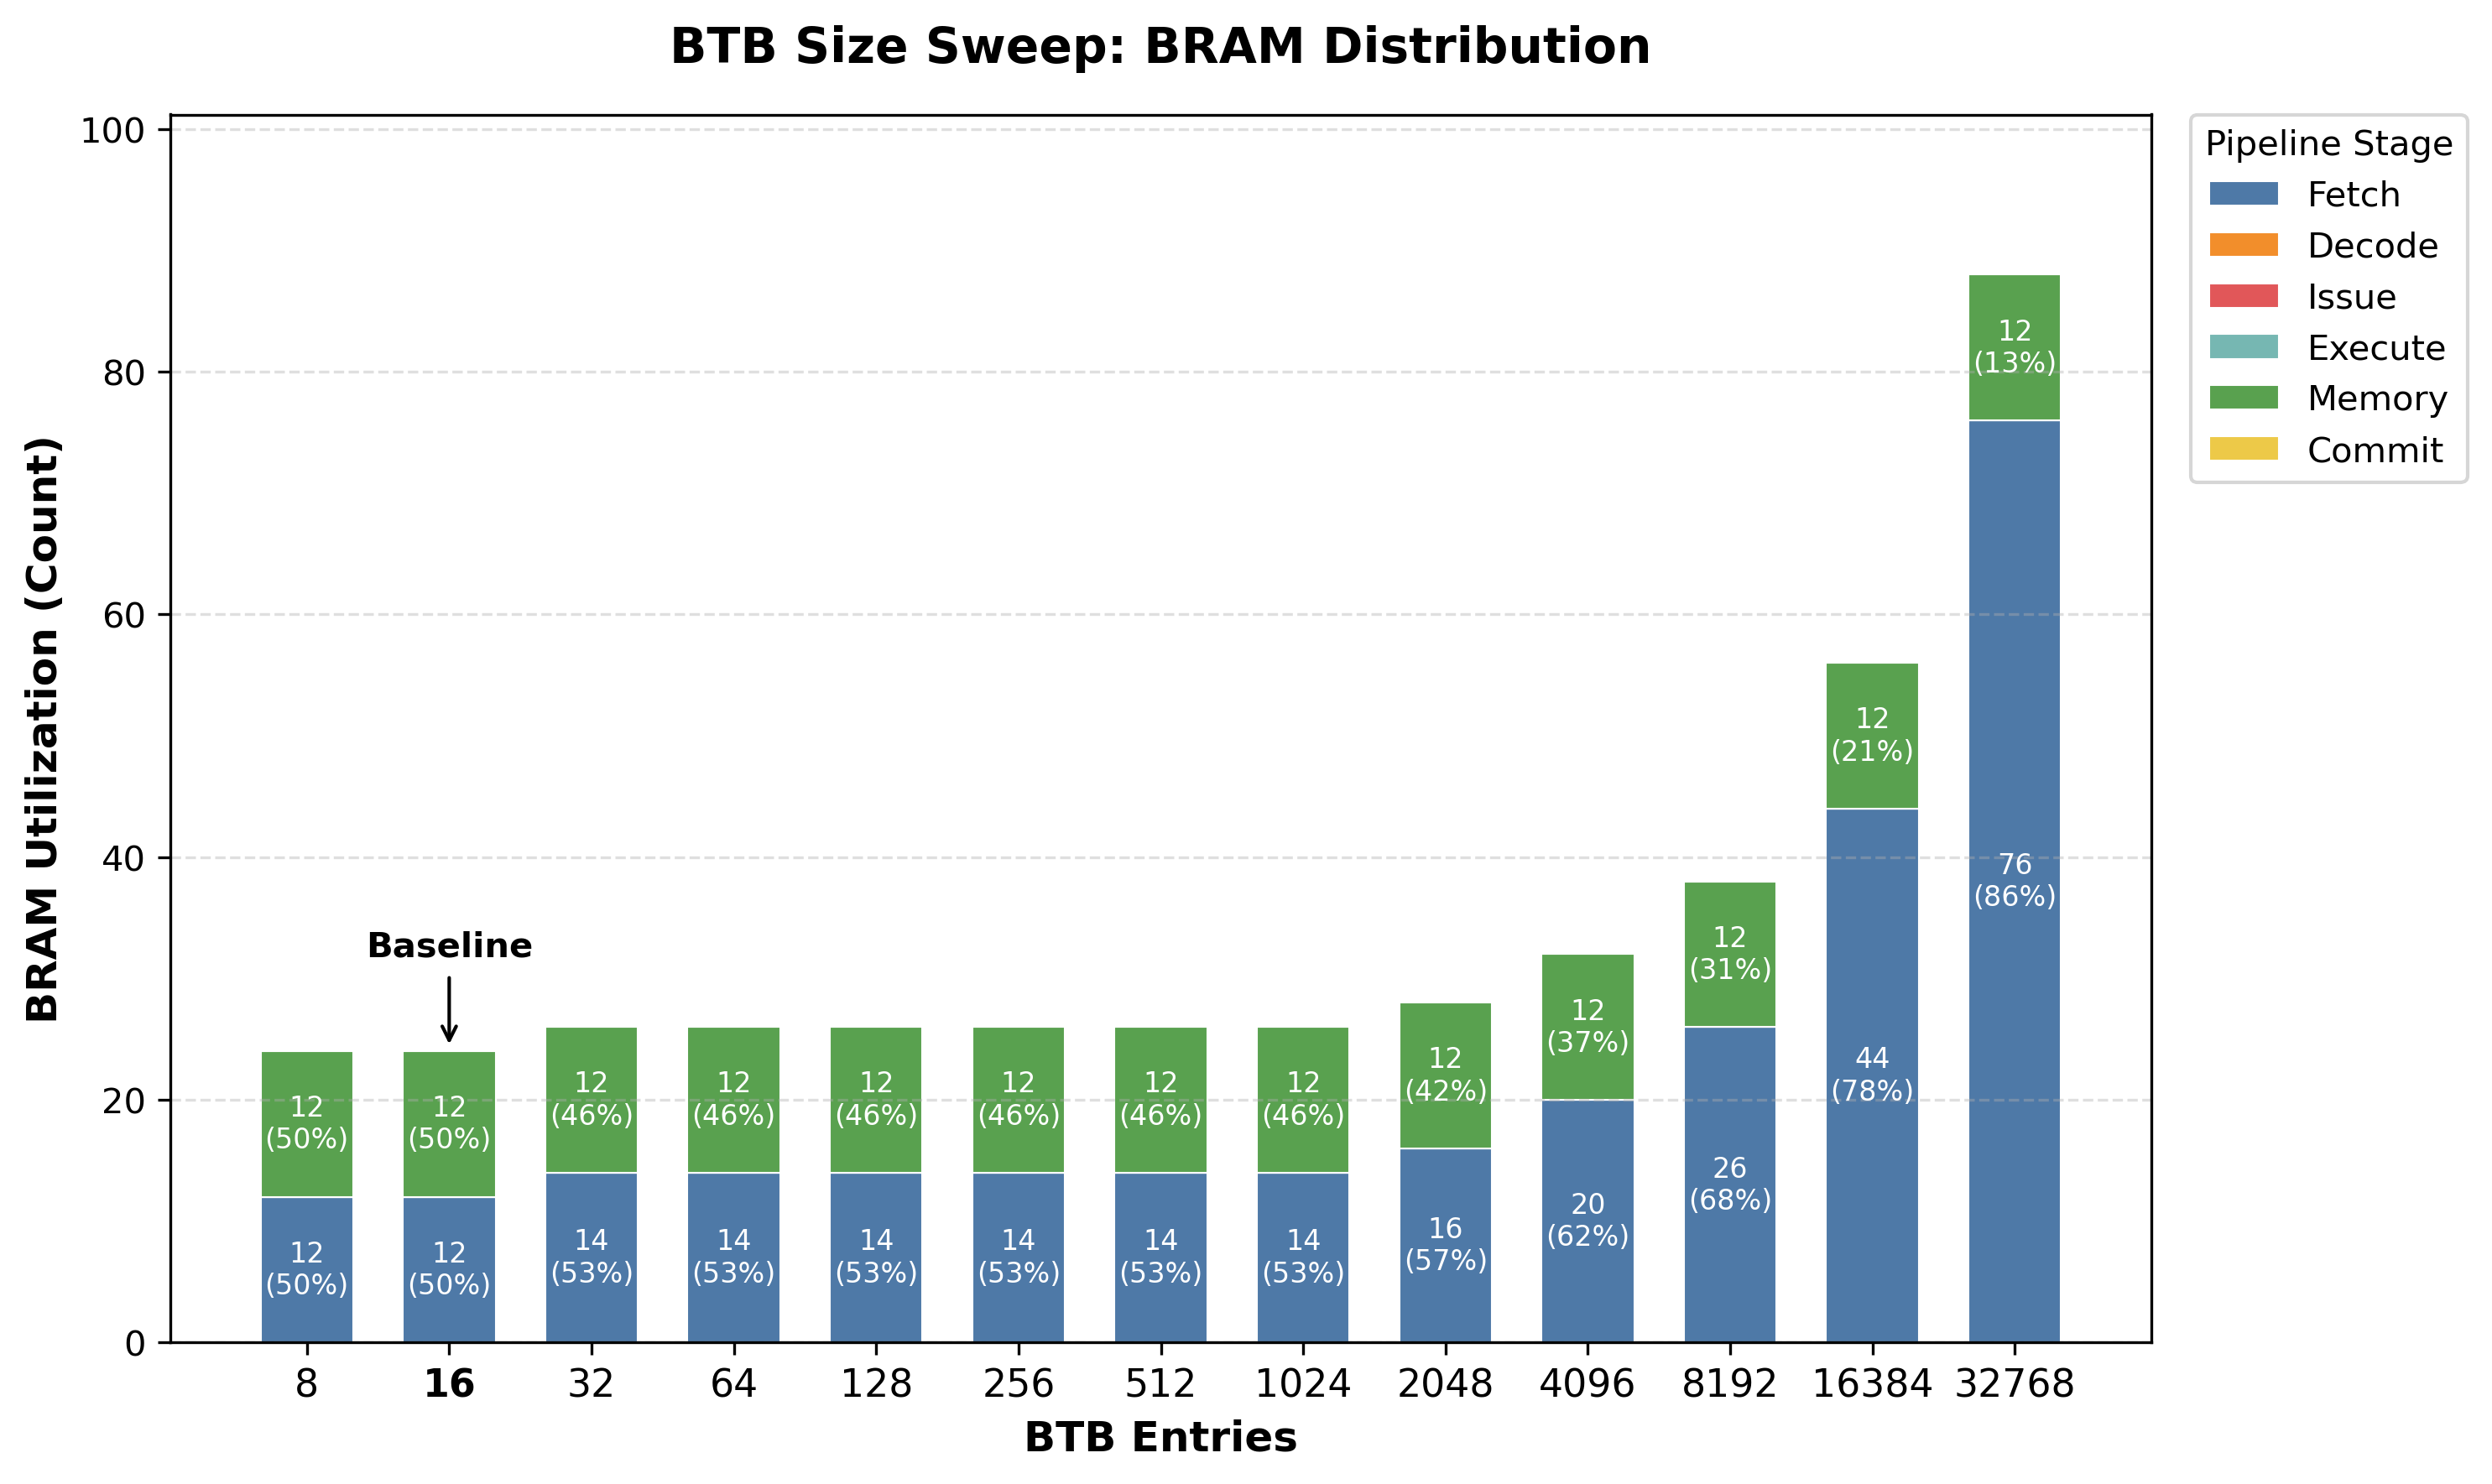
\includegraphics[angle=0,width=12.0cm]{./figures/sweep_btb_BRAM.png}
\label{fig:base_bram}
\end{center}
\end{frame}
\begin{frame}[label={sec:org1ed111a}]{Resource Usage Dynamics}
\begin{center}
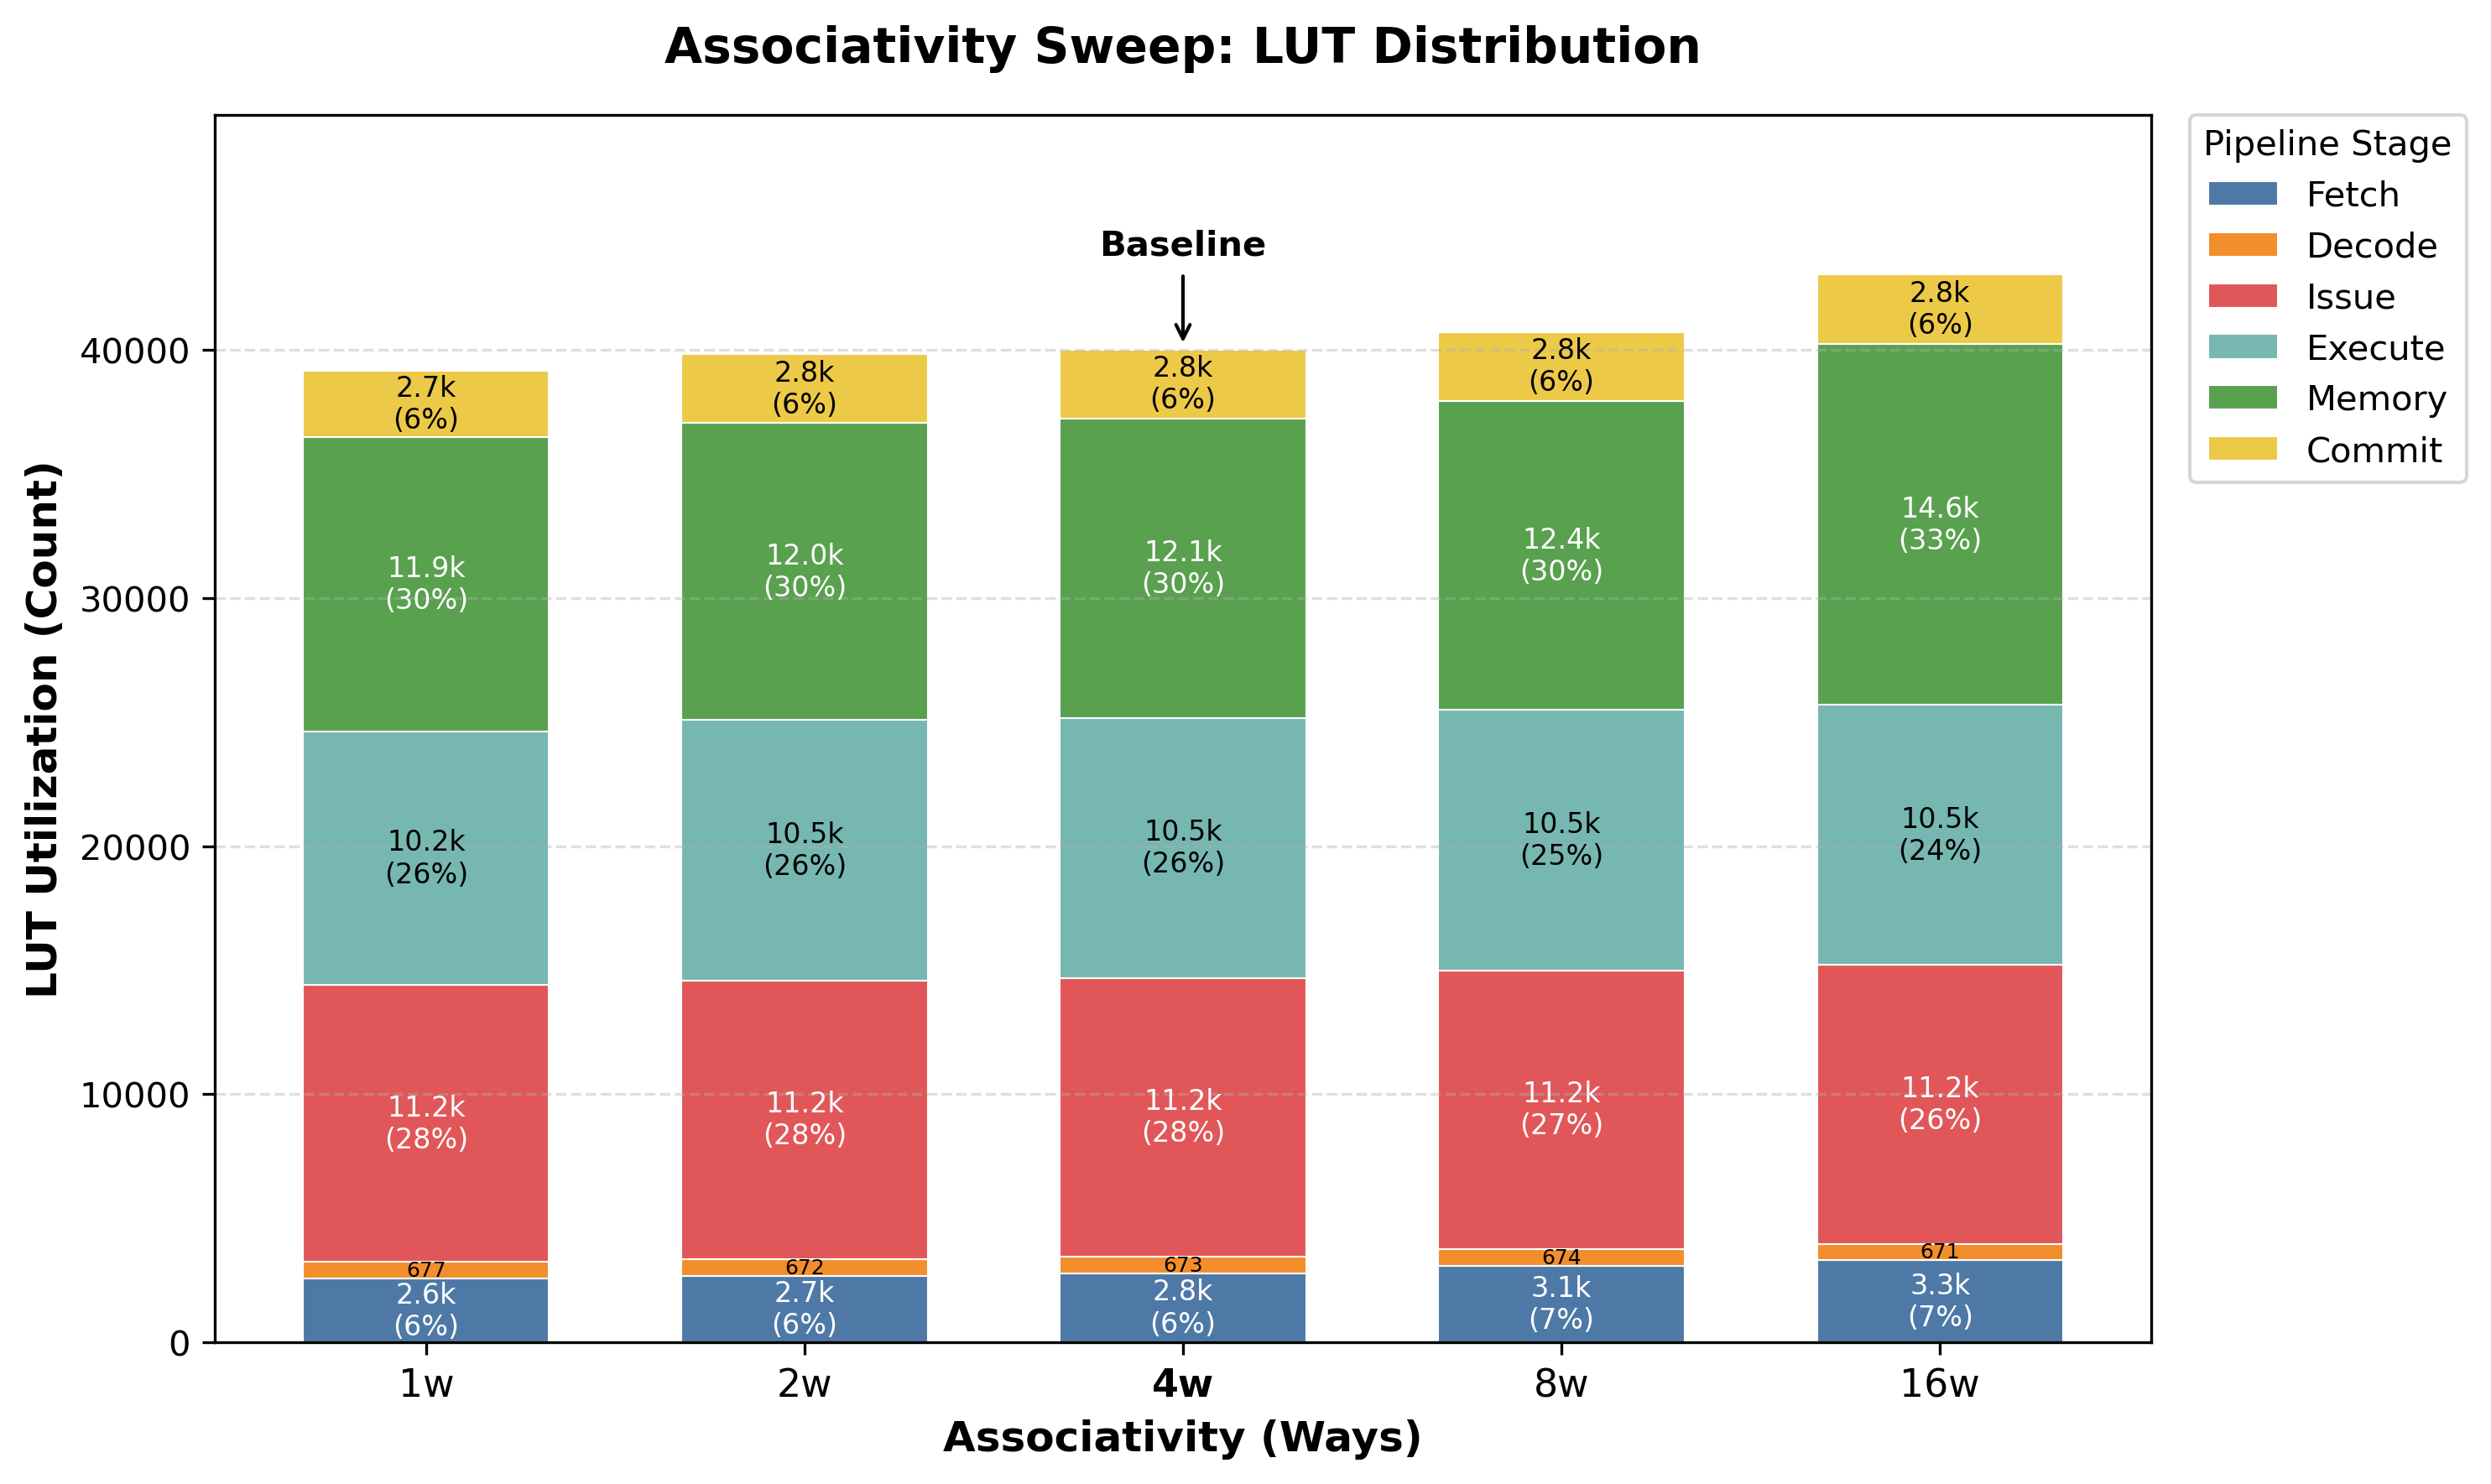
\includegraphics[angle=0,width=12.0cm]{./figures/sweep_assoc_LUT.png}
\label{fig:base_bram}
\end{center}
\end{frame}
\begin{frame}[label={sec:org2dc1421}]{Resource Usage Dynamics}
\begin{center}
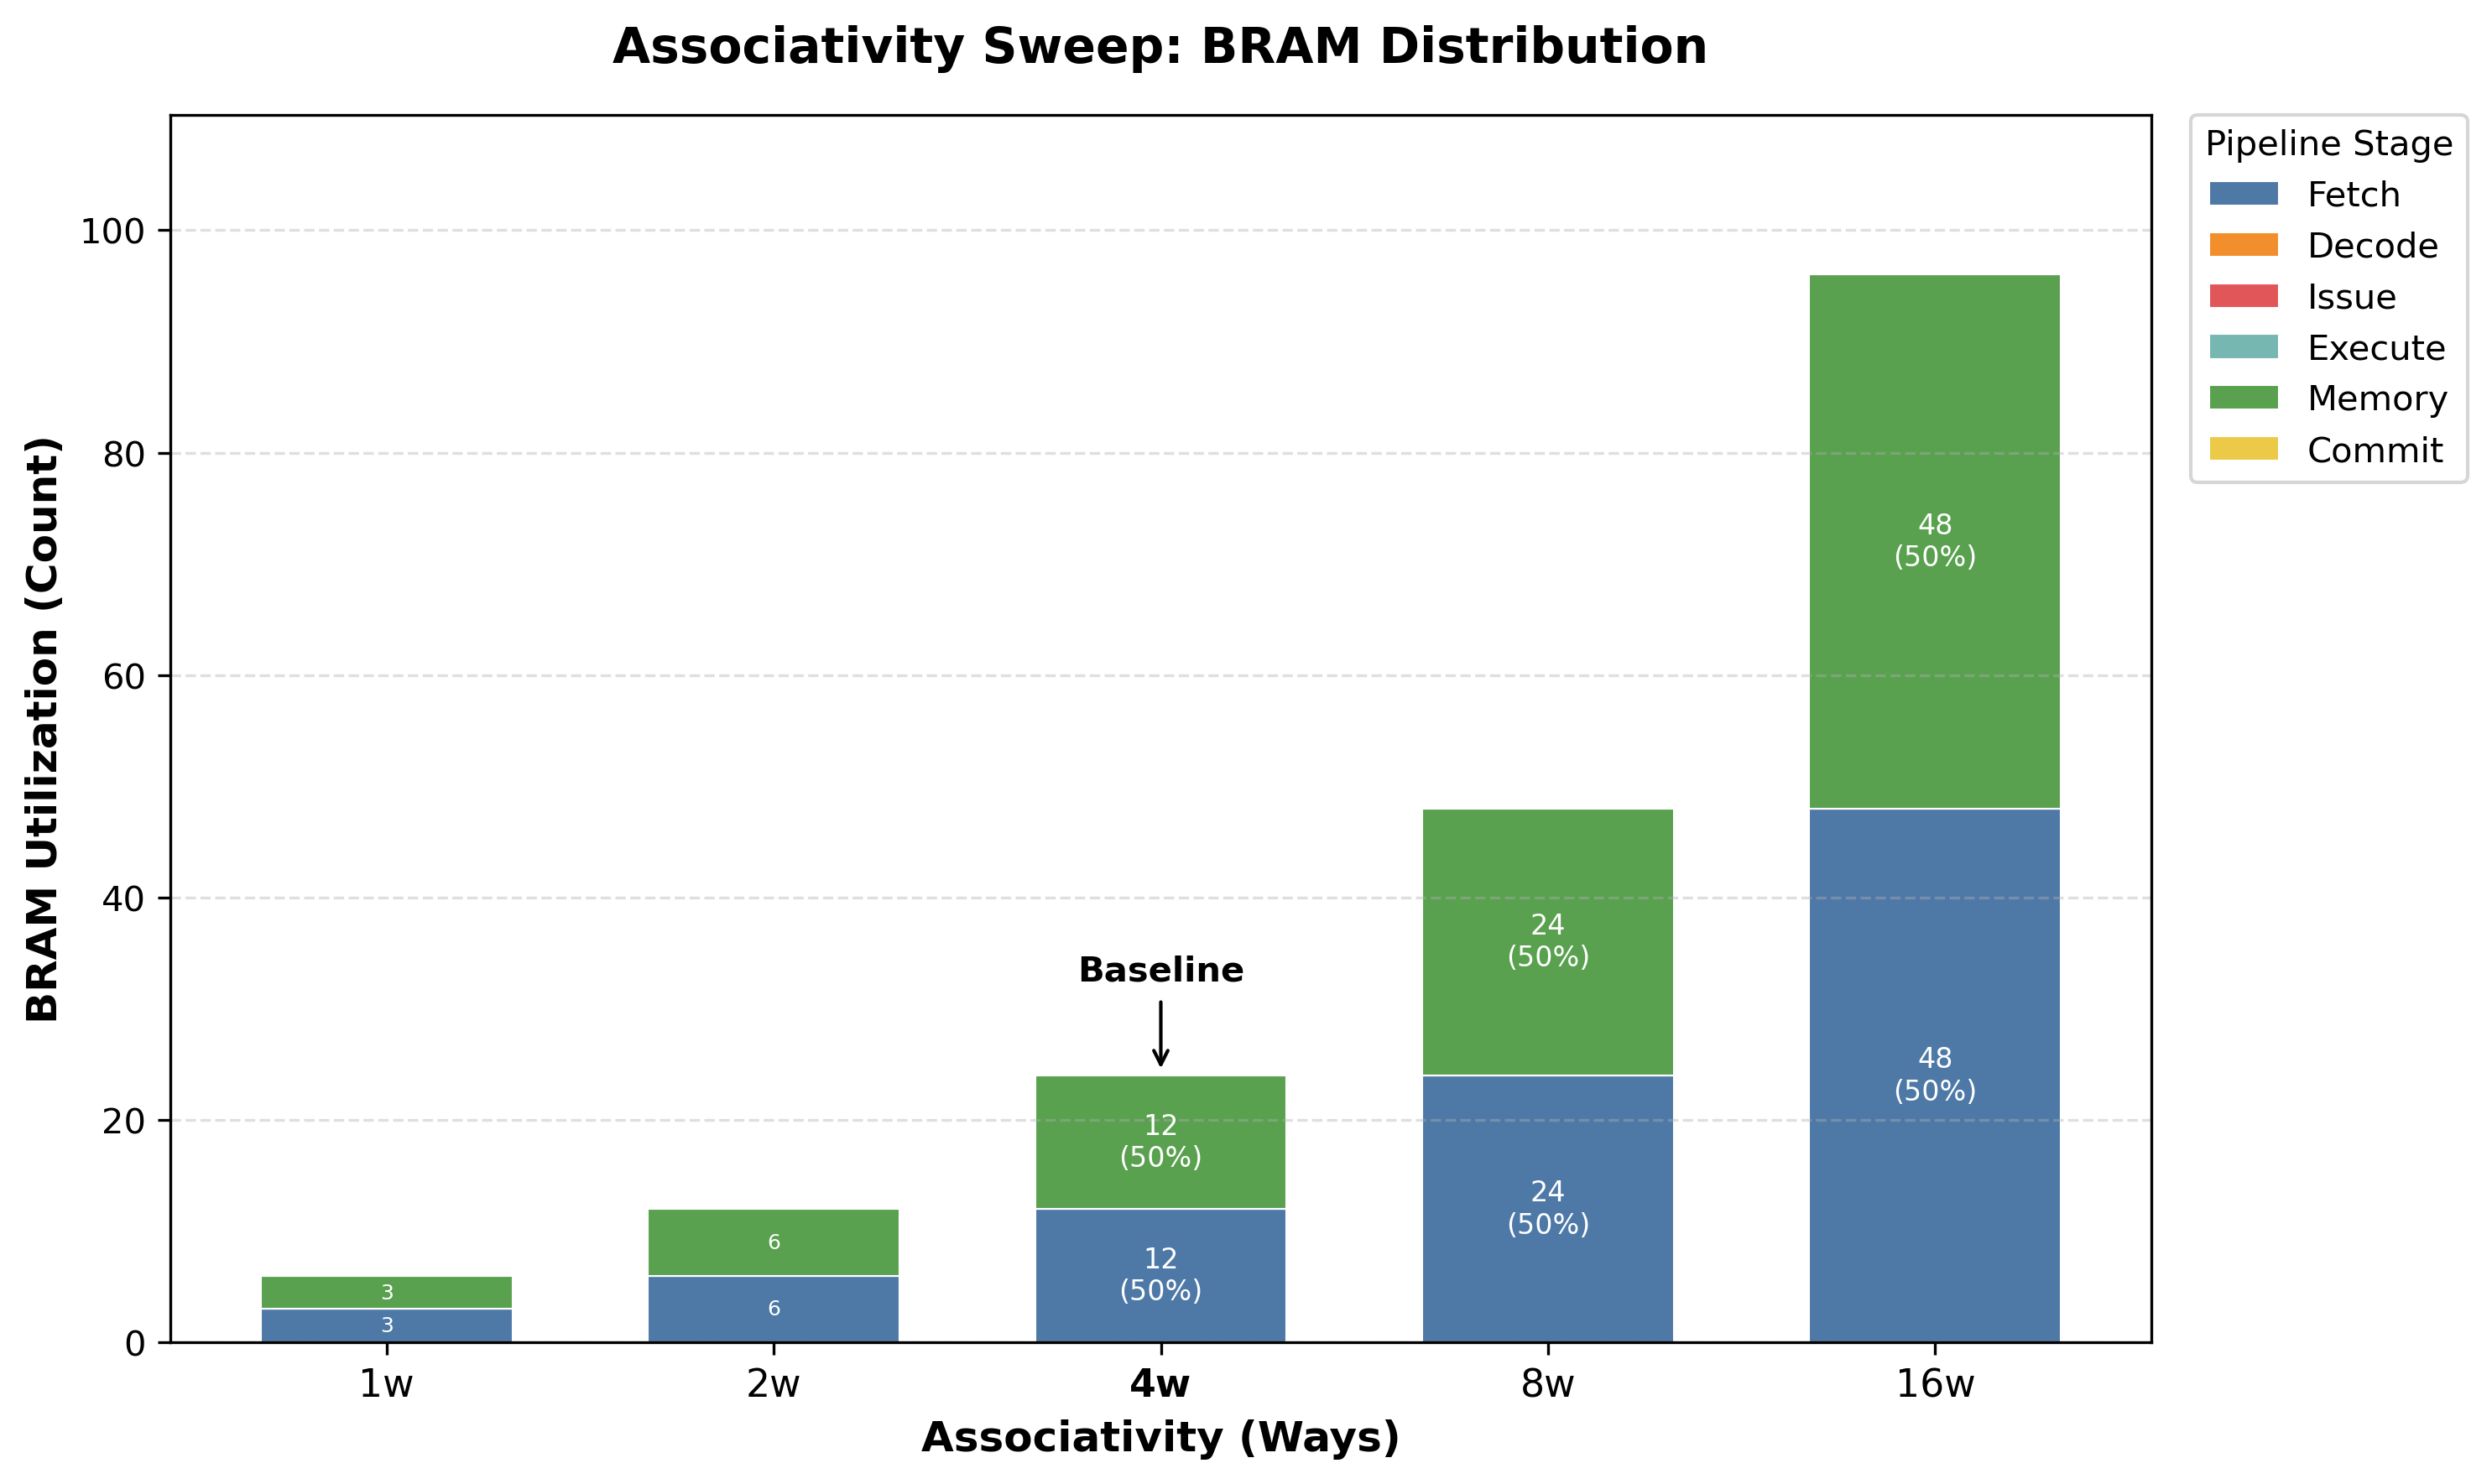
\includegraphics[angle=0,width=12.0cm]{./figures/sweep_assoc_BRAM.png}
\label{fig:base_bram}
\end{center}
\end{frame}
\begin{frame}[label={sec:org763f4d1}]{Resource Usage Dynamics}
\begin{center}
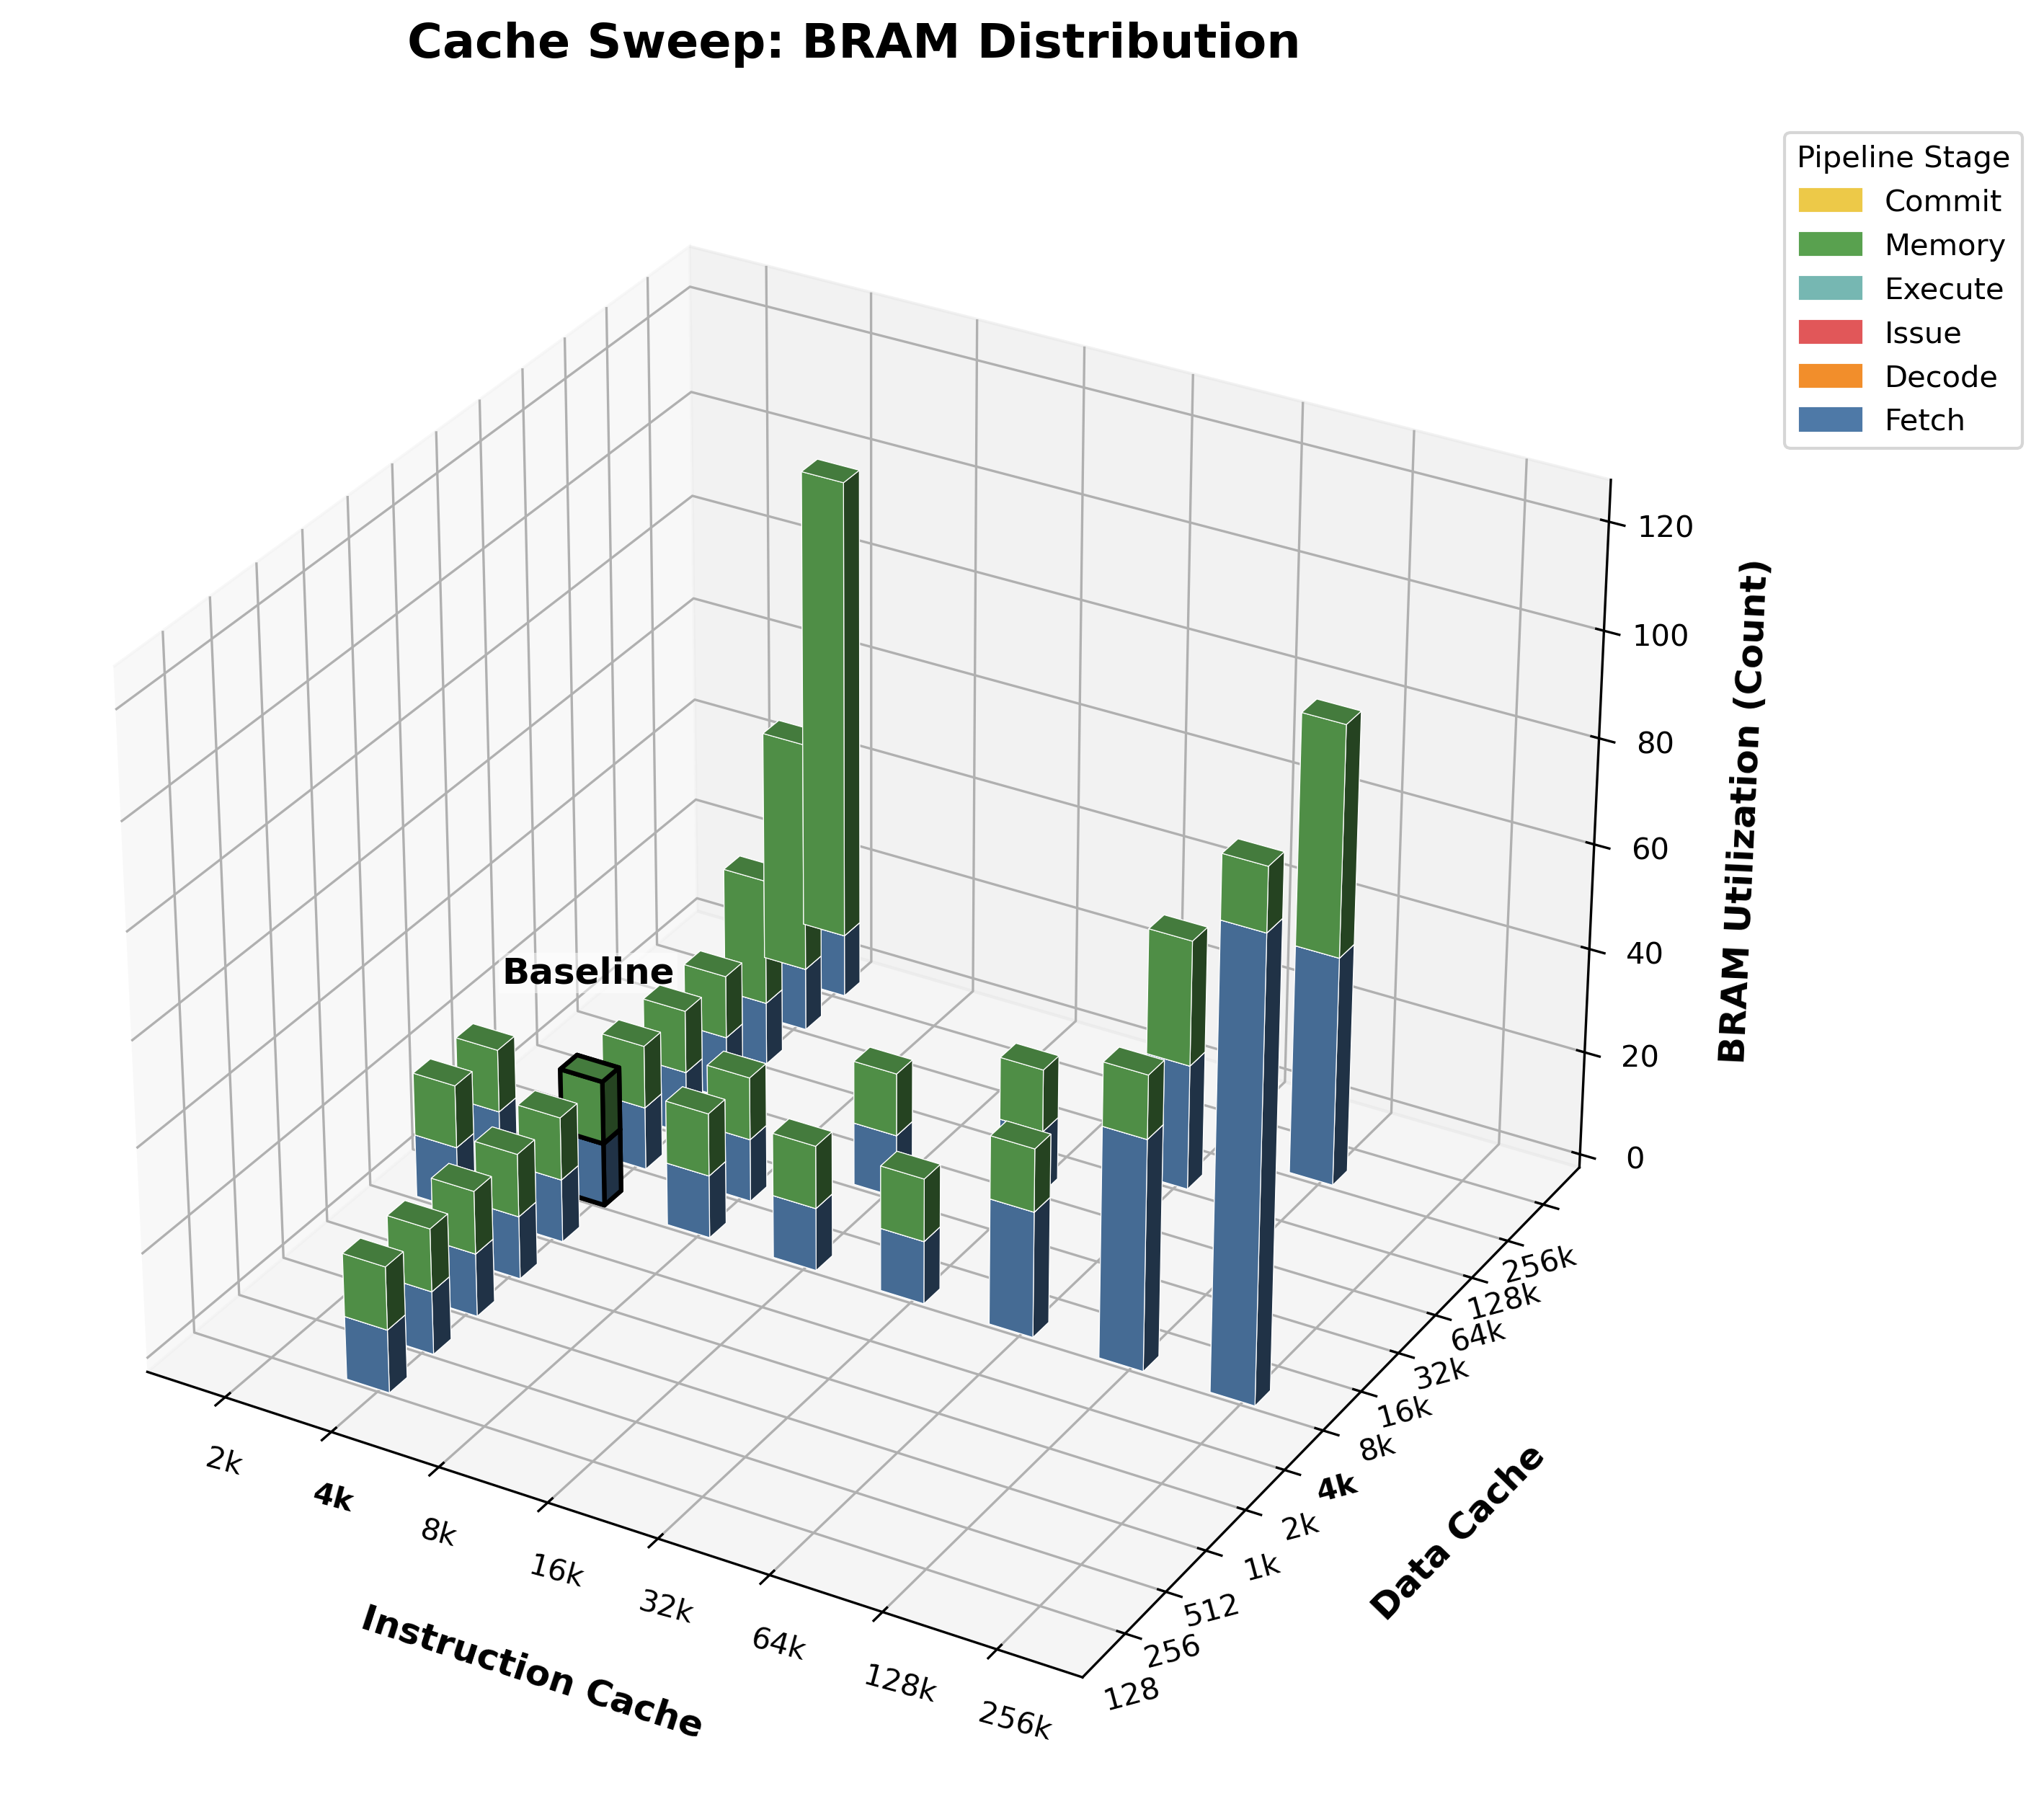
\includegraphics[angle=0,width=9.0cm]{./figures/sweep_cache_BRAM_3d.png}
\label{fig:base_bram}
\end{center}
\end{frame}
\section{Contributions}
\label{sec:org1a6a5f2}
\begin{frame}[label={sec:orgfa88dc3}]{Contributions}
\begin{itemize}
\item contributions
\begin{itemize}
\item PR the NAS repo link to the PR and the repo
\item automated script for benchmarking
\item analices in the performance
\end{itemize}
\end{itemize}
\end{frame}
\section{Conclusion and Future work}
\label{sec:org78a595a}
\begin{frame}[label={sec:org6a02c37}]{Conclusion}
\begin{itemize}
\item Conclusion
\end{itemize}
\end{frame}
\begin{frame}[label={sec:orgb8ee5f9}]{Future Work}
\begin{center}
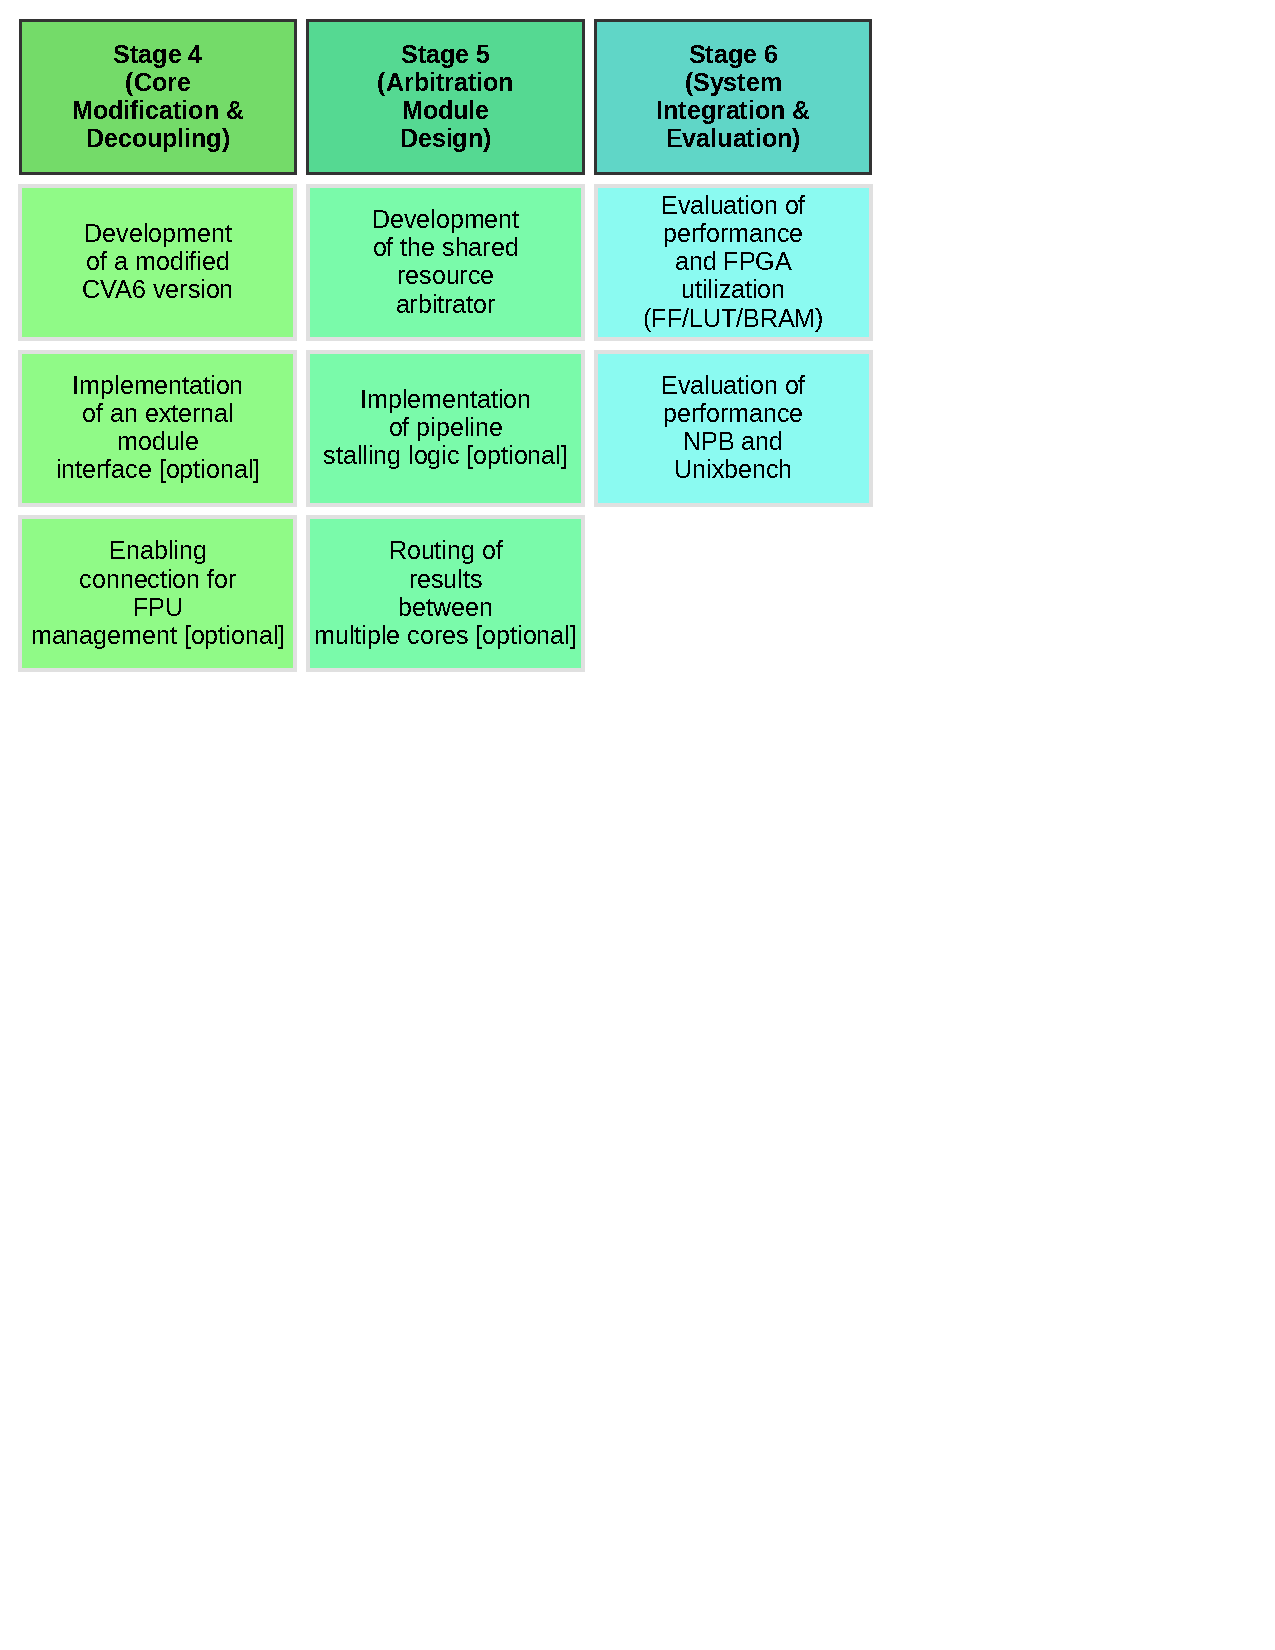
\includegraphics[trim=0 0 0 0, clip,width=\textwidth]{roadmap_future.pdf}
\label{fig:roadmap}
\end{center}
\end{frame}
\begin{frame}[label={sec:org15b8c41}]{}
\frametitle{}

\begin{huge}
\begin{center}

\textbf{\textcolor{ao-english}{Thank you!}}
\end{center}
\end{huge}

\begin{center}
\textbf{hanan.quispecondori@ip-paris.fr}

\hspace{2.5cm}

\scriptsize{\textcolor{ao-english}{This work is being supported by the \textbf{BENAGIL TEAM}}}
\end{center}

\begin{multicols}{2}

\begin{figure}
    \centering
    
\includegraphics[width=5cm]{figures/inria_logo.png}
\end{figure}

\columnbreak

\begin{figure}
    \centering
    
\includegraphics[width=1.5cm]{figures/logo_TSP.png}
\end{figure}

\end{multicols}
\end{frame}
\end{document}
